\documentclass[a4paper, 12pt, openany]{book}
\usepackage[utf8]{inputenc}
\usepackage[italian]{babel}

\usepackage[]{csvsimple}
\usepackage{float}

\usepackage{ragged2e}
\usepackage[left=25mm, right=25mm, top=15mm]{geometry}
\geometry{a4paper}
\usepackage{graphicx}
\usepackage{booktabs}
\usepackage{paralist}
\usepackage{subfig} 
\usepackage{fancyhdr}
\usepackage{amsmath}
\usepackage{amssymb}
\usepackage{amsfonts}
\usepackage{amsthm}
\usepackage{mathtools}
\usepackage{enumitem}
\usepackage{titlesec}
\usepackage{braket}
\usepackage{gensymb}
\usepackage{url}
\usepackage{hyperref}
\usepackage{csquotes}
\usepackage{multicol}
\usepackage{graphicx}
\usepackage{wrapfig}
\usepackage{caption}

\usepackage{esint}

\captionsetup{font=small}
\pagestyle{fancy}
\renewcommand{\headrulewidth}{0pt}
\lhead{}\chead{}\rhead{}
\lfoot{}\cfoot{\thepage}\rfoot{}
\usepackage{sectsty}
\usepackage[nottoc,notlof,notlot]{tocbibind}
\usepackage[titles,subfigure]{tocloft}
\renewcommand{\cftsecfont}{\rmfamily\mdseries\upshape}
\renewcommand{\cftsecpagefont}{\rmfamily\mdseries\upshape}

\let\oldsection\section% Store \section
\renewcommand{\section}{% Update \section
	\renewcommand{\theequation}{\thesection.\arabic{equation}}% Update equation number
	\oldsection}% Regular \section
\let\oldsubsection\subsection% Store \subsection
\renewcommand{\subsection}{% Update \subsection
	\renewcommand{\theequation}{\thesubsection.\arabic{equation}}% Update equation number
	\oldsubsection}% Regular \subsection

\newcommand{\abs}[1]{\left\lvert#1\right\rvert}
\newcommand{\norm}[1]{\left\lVert#1\right\rVert}
\newcommand{\vprod}[2]{\vec{#1}\times\vec{#2}}
\newcommand{\sprod}[2]{\vec{#1}\cdot\vec{#2}}

\newcommand{\g}{\text{g}}
\newcommand{\m}{\text{m}}
\newcommand{\cm}{\text{cm}}
\newcommand{\mm}{\text{mm}}
\newcommand{\s}{\text{s}}
\newcommand{\N}{\text{N}}
\newcommand{\Hz}{\text{Hz}}

\newcommand{\virgolette}[1]{``\text{#1}"}
\newcommand{\tildetext}{\raise.17ex\hbox{$\scriptstyle\mathtt{\sim}$}}

\renewcommand{\arraystretch}{1.2}

\addto\captionsenglish{\renewcommand{\figurename}{Fig.}}
\addto\captionsenglish{\renewcommand{\tablename}{Tab.}}

\DeclareCaptionLabelFormat{andtable}{#1~#2  \&  \tablename~\thetable}

\setlength{\parindent}{0pt}

\newcommand{\dive}{\nabla\cdot}
\newcommand{\rot}{\nabla\times}

\graphicspath{{./images/}}

\author{Leonardo Cerasi%
	\thanks{\scriptsize\href{mailto:leonardo.cerasi@studenti.unimi.it}{leo.cerasi@pm.me}}%
	, Lucrezia Bioni\\
	\small GitHub repository: \href{https://github.com/LeonardoCerasi/notes}{LeonardoCerasi/notes}}
\title{\Huge\textbf{Geometria e Gruppi 1} \\ \large Prof. A. Zaccone, a.a. 2024-25}

\begin{document}

\frontmatter

\maketitle
\tableofcontents

\mainmatter

\part{Geometria}

\chapter{Tensori}
\selectlanguage{italian}

\section{Sistemi di coordinate e trasformazioni}


Le leggi fisiche sono equazioni che coinvolgono quantità invarianti rispetto a cambiamenti di sistemi di riferimento (RF): queste quantità sono espresse tramite tensori, oggetti che ubbidiscono a determinate leggi di trasformazione nel passaggio da un RF a un altro. \\ 
I tensori sono generalmente delle funzioni spaziali, ovvero dipendono da set ordinati di coordinate spaziali (quantità misurabili sperimentalmente, dunque fisiche, non solo matematiche). Le coordinate spaziali designano un punto nello spaziotempo che, di per sé, è assoluto: utilizzando diversi sistemi di riferimento, però, esso sarà descritto da set di coordinate differenti, sebbene la sua esistenza sia slegata da essi.

\begin{definition}
	Dato uno spazio o una sua regione costituita da punti, descritti da $ n $-ple ordinate di variabili continue $ \{x^k\}_{k=1,\dots,n}\subset\R, n \in \N $, si definisce \textit{trasformazione ammissibile} un insieme di funzioni $ y^k = y^k (x^1, \dots, x^n), k = 1, \dots, n $ che soddisfino le seguenti condizioni:
	\begin{enumerate}
		\item $ y^k (x^1, \dots, x^n) $ è monodroma (single-valued) e continuamente derivabile $ \forall k = 1, \dots, n $;
		\item $ \det \left[ \frac{\pa y^k}{\pa x^j} \right] \neq 0 $.
	\end{enumerate}
\end{definition}

La condizione sulla Jacobiana è necessaria per garantire l'invertibilità della trasformazione. 

\begin{definition}
	Si definisce \textit{tensore} di rango $ r+s $ un oggetto con $ r+s $ componenti dipendenti dalle coordinate $ x^k $:
	\begin{equation}
		T^{\,i_1 \dots i_r}_{j_1 \dots j_s} = T^{\,i_1 \dots i_r}_{j_1 \dots j_s} (x^1, \dots, x^n)
		\label{eq:1}
	\end{equation}
	dove ciascun indice varia in $ \{1, \dots, n\} $.
\end{definition}
Si adottano inoltre le seguenti convenzioni sugli indici:
\begin{enumerate}
	\item Einstein's summation convention: $ A^k B_k \equiv \sum_{k = 1}^{n} A^k B_k $;
	\item range convention: ogni indice libero in un'equazione varia indipendentemente in $ \{1, \dots, n\} $, quindi se in un'equazione sono presenti $ N $ indici liberi, essa rappresenta $ n^N $ equazioni distinte;
	\item in $ \frac{\pa y^k}{\pa x^j} $ l'indice $ j $ è considerato un petice.
\end{enumerate}

\begin{definition}
	Data una trasformazione ammissibile delle coordinate ed un tensore, si definisce la \textit{trasformazione indotta} delle componenti del tensore:
	\begin{equation}
		\tilde{T}^{\,i_1 \dots i_r}_{j_1 \dots j_s} (y^1, \dots, y^n) = \tilde{T}^{\,i_1 \dots i_r}_{j_1 \dots j_s} \left[ T^{1 \dots 1}_{1 \dots 1} (x^1, \dots, x^n), \dots, T^{\,n \dots n}_{n \dots n} (x^1, \dots, x^n) \right]
		\label{eq:2}
	\end{equation}
\end{definition}

È possibile dimostrare i seguenti asserti:

\begin{theorem}
	Esiste un \textnormal{isomorfismo} tra una trasformazione di coordinate e la sua trasformazione indotta.
\end{theorem}

\begin{proposition}
	Ogni trasformazione indotta è un isomorfismo.
\end{proposition}

In generale, i tensori sono definiti dalle loro leggi di trasformazione indotte, che possono essere lineari o non-lineari (ad esempio nel caso di RF curvilinei), ma sempre omogenee. \\
Nel seguito verranno considerati solo tensori che sono funzioni $ \R^n \longrightarrow \R^{n^{r+s}} $.


\subsection{Tensori assoluti}


\begin{definition}
	Si definisce \textit{scalare} un tensore $ \alpha (x^1, \dots, x^n) $ di rango $ 0 $ con legge di trasformazione:
	\begin{equation}
		\tilde{\alpha} (y^1, \dots, y^n) = \alpha (x^1, \dots, x^n)
		\label{eq:3}
	\end{equation}
\end{definition}

Il valore di un campo scalare in un punto dello spazio è (giustamente) indipendente dal RF.

\begin{definition}
	Si definisce \textit{vettore contravariante} un tensore $ a^k (x^1, \dots, x^n) $ di rango $ 1 $ con legge di trasformazione:
	\begin{equation}
		\tilde{a}^k (y^1, \dots, y^n) = \frac{\pa y^k}{\pa x^j} a^j (x^1, \dots, x^n)
		\label{eq:4}
	\end{equation}
\end{definition}

\begin{definition}
	Si definisce \textit{vettore covariante} un tensore $ a_k (x^1, \dots, x^n) $ di rango $ 1 $ con legge di trasformazione:
	\begin{equation}
		\tilde{a}_k (y^1, \dots, y^n) = \frac{\pa x^j}{\pa y^k} a_j (x^1, \dots, x^n)
		\label{eq:5}
	\end{equation}
\end{definition}

Per ricavare le due leggi di trasformazione, va ricordato l'isomorfismo canonico tra uno spazio vettoriale $ V $ ed il suo duale $ V^* $: grazie ad esso, un generico vettore $ \mathbf{v} $ può essere espresso sia sulla base canonica $ \{\mathbf{b}_i\}_{i=1,\dots,n} $ di $ V $ come $ \mathbf{v} = v^i \mathbf{b}_i $, sia sulla base duale $ \{\mathbf{b}^i\}_{i=1,\dots,n} $ di $ V^* $ come $ \mathbf{v} = v_i \mathbf{b}^i $. \\ 
%
Considerando uno spazio euclideo con RF $ (x^1, \dots, x^n) $, la base canonica dello spazio in un punto $ \mathbf{r} $ è data da $ \mathbf{e}_i = \frac{\pa \mathbf{r}}{\pa x^i} $, dunque, dato che $ \mathbf{a} = a^j \mathbf{e}_j = \tilde{a}^k \tilde{\mathbf{e}}_k $:

\begin{equation}
	\mathbf{e}_j = \frac{\pa \mathbf{r}}{\pa x^j} = \frac{\pa y^k}{\pa x^j} \frac{\pa \mathbf{r}}{\pa y^k} = \frac{\pa y^k}{\pa x^j} \tilde{\mathbf{e}}_k \quad \Longrightarrow \quad \tilde{a}^k = \frac{\pa y^k}{\pa x^j} a^j
	\label{eq:6}
\end{equation}

Se invece si esprime $ \mathbf{a} $ sulla base duale $ \mathbf{e}^i = \nabla x^i $, dato che $ \mathbf{a} = a_j \mathbf{e}^j = \tilde{a}_k \tilde{\mathbf{e}}^k $:

\begin{equation}
	\mathbf{e}^j = \frac{\pa x^j}{\pa \mathbf{r}} = \frac{\pa x^j}{\pa y^k} \frac{\pa y^k} {\pa \mathbf{r}} = \frac{\pa x^j}{\pa y^k} \tilde{\mathbf{e}}^k \quad \Longrightarrow \quad \tilde{a}_k = \frac{\pa x^j}{\pa y^k} a_j
	\label{eq:7}
\end{equation}
Si può notare che la legge di trasformazione contravariante è quella del differenziale, mentre quela covariante è quella del gradiente. \\
%
È possibile generalizzare queste leggi di trasformazioni a tensori qualsiasi.

\begin{definition}
	Dato un tensore $ T^{\,i_1 \dots i_r}_{j_1 \dots j_s} (x^1, \dots, x^n) $ di rango $ r+s $, la sua legge di trasformazione è:
	\begin{equation}
		\tilde{T}^{\,i_1 \dots i_r}_{j_1 \dots j_s} (y^1, \dots, y^n) = \frac{\pa y^{i_1}}{\pa x^{k_1}} \dots \frac{\pa y^{i_r}}{\pa x^{k_r}} \frac{\pa x^{l_1}}{\pa y^{j_1}} \dots \frac{\pa x^{l_s}}{\pa y^{l_s}} T^{k_1 \dots k_r}_{l_1 \dots l_s} (x^1, \dots, x^n)
		\label{eq:8}
	\end{equation}
\end{definition}

\begin{example}
	Un esempio interessante è il tensore di Kronecker, definito a partire dalla delta di Kronecker: $ \tilde{\delta}^i_j = \frac{\pa y^i}{\pa x^k} \frac{\pa x^l}{\pa y^j} \delta^k_l = \frac{\pa y^i}{\pa y^j} = \delta^i_l $, dunque è un tensore isotropico (indipendente dal RF).
\end{example}

\begin{example}
	Un altro esempio di tensore è il campo elettrico, definito come il gradiente di un campo scalare (anche esso tensore di rango $ 0 $): $ \mathbf{E} = -\nabla\phi $, ovvero $ E_i = - \frac{\pa \phi}{\pa x^i} $.
\end{example}

\begin{example}
	Un tensore di rango $ 2 $ può essere ottenuto, ad esempio, come prodotto diretto tra due tensori di rango $ 1 $: ad esempio $ \tens{T} = \mathbf{v} \otimes \mathbf{u} $, che può essere espresso in tre modi:
	\begin{enumerate}
		\item contravariante: $ \tens{T} = v^j \mathbf{e}_j \otimes u^k \mathbf{e}_k $, quindi $ T^{jk} = v^j u^k $;
		\item covariante: $ \tens{T} = v_j \mathbf{e}^j \otimes u_k \mathbf{e}^k $, quindi $ T_{jk} = v_j u_k $;
		\item mixed: $ \tens{T} = v_j \mathbf{e}^j \otimes u^k \mathbf{e}_k $, quindi $ T_j^k = v_j u^k $.
	\end{enumerate}
\end{example}

\begin{example}
	Anche il gradiente di un vettore è un tensore di rango $ 2 $, poiché può essere visto come prodotto diretto: $ \tens{T} = \nabla\mathbf{v} $, ovvero $ T^{\,i}_j = \frac{\pa v^i}{\pa x^j} $.
\end{example}


\subsection{Pseudotensori}


Un particolare tipo di trasformazioni di coordinate sono le rotazioni in $ \R^3 $.

\begin{definition}
	Si definisce \textit{rotazione} un'isometria di $ \R^3 $ rappresentata da una matrice ortogonale $ \tens{R} \in \Ot \defeq \{\tens{R} \in \R^{3\times3} : \tens{R}^{\intercal}\tens{R} = \tens{R}\tens{R}^{\intercal} = \tens{I}_3 \} $.
\end{definition}

È necessario fare una distinzione tra due classi di rotazioni.

\begin{definition}
	Si definisce \textit{rotazione propria} una rotazione rappresentata da una matrice ortogonale $ \tens{R} \in \SOt \defeq \{\tens{R} \in \Ot : \det\tens{R} = +1 \} $.
\end{definition}

\begin{example}
	Considerando un tensore di rango $ 2 $ definito come $ \tens{T} = \ve{v} \otimes \ve{u} $ ed una rotazione propria $ \tens{R} $: $ \tens{T} = T^i_j \ve{e}_i \otimes \ve{e}^j = \tilde{T}^i_j \tilde{\ve{e}}_i \otimes \tilde{\ve{e}}^j $, ma $ \ve{e}^j = \frac{\pa x^j}{\pa y^k} \tilde{\ve{e}}^k $, dunque $ \tilde{T}^i_j = \frac{\pa y^i}{\pa x^k} \frac{\pa x^l}{\pa y^j} T^k_l $; dato che il Jacobiano della trasformazione è proprio la matrice di rotazione $ \tens{R} $, si vede che le componenti contravarianti del tensore trasformano secondo $ \tens{R} $, mentre le componenti covarianti secondo $ \tens{R}^{-1} = \tens{R}^{\intercal} $.
\end{example}

\begin{definition}
	Si definisce \textit{rotazione impropria} una rotazione rappresentata da una matrice ortogonale $ \tens{R} \in \Ot : \det\tens{R} = -1 $.
\end{definition}

Le rotazioni improprie sono rotazioni con l'inversione di un asse, dunque non conservano l'orientazione (handedness) dello spazio.

\begin{definition}
	Si definisce \textit{pseudotensore} di rango $ r+s $ un oggetto tensoriale di rango $ r+s $ che per effetto di una rotazione trasforma secondo:
	\begin{equation}
		\tilde{T}^{\,i_1 \dots i_r}_{j_1 \dots j_s} (y^1, \dots, y^n) = \left(\det\tens{R}\right)\, \frac{\pa y^{i_1}}{\pa x^{k_1}} \dots \frac{\pa y^{i_r}}{\pa x^{k_r}} \frac{\pa x^{l_1}}{\pa y^{j_1}} \dots \frac{\pa x^{l_s}}{\pa y^{l_s}} T^{k_1 \dots k_r}_{l_1 \dots l_s} (x^1, \dots, x^n)
		\label{eq:9}
	\end{equation}
\end{definition}

Uno pseudotensore acquista un segno $ - $ sotto rotazioni improprie. \\
Lo pseduotensore per eccellenza è il tensore di Levi-Civita.

\begin{definition}
	Si definisce il tensore di Levi-Civita nel caso tridimensionale euclideo:
	\begin{equation}
		\epsilon_{ijk} = \epsilon^{ijk} = 
		\begin{cases}
			+1 &\quad (i,j,k) = \sigma_p(1,2,3) \\
			-1 &\quad (i,j,k) = \sigma_d(1,2,3) \\
			0  &\quad \text{altrimenti}
		\end{cases}
		\label{eq:10}
	\end{equation}
	dove $ \sigma_{p,d} $ sono delle permutazioni pari/dispari.
\end{definition}

È possibile dimostrare le seguenti proposizioni.

\begin{proposition}\label{levi-civ-det}
	Data $ \tens{A} \in \R^{3\times 3} $, si ha $ \left(\det\tens{A}\right)\, \epsilon_{lmn} = A_{li} A_{mj} A_{nk} \epsilon^{ijk} $.
\end{proposition}

\begin{proposition}\label{epsilon-delta}
	$ \epsilon_{ijk}\epsilon_{klm} = \delta_{il}\delta_{jm} - \delta_{im}\delta_{jl}.$
\end{proposition}

Dalla prop. \ref{levi-civ-det} è facile ricavare la legge di trasformazione del tensore di Levi-Civita:
\begin{equation}
	\tilde{\epsilon}_{ijk} = \frac{\pa x^l}{\pa y^i} \frac{\pa x^m}{\pa y^j} \frac{\pa x^n}{\pa y^k} \epsilon_{lmn} = \left(\det\tens{R}^{-1}\right) \epsilon_{ijk} = \left(\det\tens{R}\right) \epsilon_{ijk}
	\label{eq:11}
\end{equation}
Quindi sotto rotazioni improprie il tensore di Levi-Civita cambia di segno.

\begin{example}
	Dato che $ B^i = \left(\nabla\times\ve{A}\right)^i = \epsilon^{ijk}\frac{\pa A_k}{\pa x^j}$, si vede che, per effetto di rotazioni improprie, il campo magnetico cambia di segno: ciò è legato al cambiamento di handedness dello spazio.
\end{example}


\subsection{Tensore Metrico}


Mentre nel caso euclideo la base canonica $ \ve{e}_j = \frac{\pa \ve{r}}{\pa x^j} $ ($ \ve{e}_j $ tangente alla $ j $-esima linea coordinata) coincide con la base duale $ \ve{e}^j = \nabla x^j $ ($ \ve{e}^j $ ortogonale alla $ j $-esima linea coordinata), ciò non è valido in generale.\\
In RF generici, per passare da una base alla sua duale è necessario introdurre un oggetto tensoriale detto tensore metrico.

\begin{definition}
	Data una base $ \{\ve{e}_j\}_{j=1,\dots,n} $, si definisce il \textit{tensore metrico} in tale base come $ g_{ij} \defeq \ve{e}_i \cdot \ve{e}_j \, \forall i,j = 1,\dots,n$.
\end{definition}

Ovviamente è possibile specificare le componenti controvarianti $ g^{ij} $, al posto di quelle covarianti. \\
Nel caso in cui i vettori base sono mutualmente ortogonali, il tensore metrico sarà rappresentato da una matrice diagonale: come negli spazi vettoriali si può sempre ottenere una base ortonormale da una base non-ortonormale (algoritmo di Gram-Schmidt), così si può diagonalizzare anche il tensore metrico.

\begin{proposition}
	$ ds^2 = g_{ij} dx^i dx^j $.
\end{proposition}
\begin{proof}
	$ ds^2 \equiv d\ve{r} \cdot d\ve{r} = dx^i \ve{e}_i \cdot dx^j \ve{e}_j = g_{ij} dx^i dx^j $.
\end{proof}

\begin{proposition}
	Nel caso tridimensionale $ dV = \sqrt{\det\tens{g}}\, dx^1 dx^2 dx^3 $.
\end{proposition}
\begin{proof}
	Considerando una base già ortogonalizzata tale che $ g_{ij} = h_i^2 \delta_{ij} $, dove $ h_i $ è detto fattore scala, abbiamo $ ds^2 = h_i^2 (dx^i)^2 $ (concorde col fatto che $ d\ve{r} = \frac{\pa \ve{r}}{\pa x^j} dx^j = h_j dx^j \hat{\ve{e}}_j $ per definizione di $ \hat{\ve{e}}_j $); per definizione $ dV = \abs{dx^1\ve{e}_1 \cdot (dx^2\ve{e}_2 \times dx^3\ve{e}_3)} = h_1 h_2 h_3 dx^1 dx^2 dx^3 \hat{\ve{e}}_1 \cdot (\hat{\ve{e}}_2 \times \hat{\ve{e}}_3) $, ma la base è ortogonale e per il tensore metrico si ha $ \det\tens{g} = h_1^2 h_2^2 h_3^2 $, dunque $ dV = \sqrt{\det\tens{g}}\, dx^1 dx^2 dx^3 $.
\end{proof}

Il tensore metrico è dunque fondamentale per il calcolo di distanze, aree, volumi, etc., ma ha anche un'altra importante funzione: passare dalle componenti covarianti a quelle contravarianti e viceversa.\\
Il prodotto scalare può essere espresso in vari modi: $ \ve{a}\cdot\ve{b} = a_i b^i = a^i b_i = g_{ij} a^i b^j = g^{ij} a_i b_j $, dunque si notano due importanti identità:

\begin{equation}
	\begin{split}
		g_{ij} a^i &= a_j \\
		g^{ij} a_i &= a^j
	\end{split}
	\label{eq:12}
\end{equation}

È dunque possibile passare da una base al suo duale mediante contrazione col tensore metrico.

\begin{proposition}
	$ \left[g^{ij}\right] = \left[g_{ij}\right]^{-1} $.
\end{proposition}
\begin{proof}
	$ a^i = g^{ij} a_j = g^{ij} g_{jk} a^k $, dunque $ g^{ij} g_{jk} = \delta^i_k $, ovvero $ \left[g^{ij}\right]\left[g_{ij}\right] = \tens{I}_n $.
\end{proof}

Da questa dimostrazione si nota che $ g^i_j = \delta^i_j $.\\
Data la relazione di passaggio tra componenti covarianti e contravarianti, è possibile enunciare in maniera generica la legge di trasformazione di un tensore.

\begin{definition}
	Dato un tensore $ T^{\,i_1 \dots i_r}_{j_1 \dots j_s} (x^1, \dots, x^n) $ di rango $ r+s $, la sua legge di trasformazione è:
	\begin{equation}
		\tilde{T}^{\,i_1 \dots i_r}_{j_1 \dots j_s} (y^1, \dots, y^n) = \det\left[\frac{\pa x}{\pa y}\right]^w \frac{\pa y^{i_1}}{\pa x^{k_1}} \dots \frac{\pa y^{i_r}}{\pa x^{k_r}} \frac{\pa x^{l_1}}{\pa y^{j_1}} \dots \frac{\pa x^{l_s}}{\pa y^{l_s}} T^{k_1 \dots k_r}_{l_1 \dots l_s} (x^1, \dots, x^n)
		\label{eq:13}
	\end{equation}
	dove in base al valore di $ w $ si parla di:
	\begin{itemize}
		\item $ w = 0 $: tensore assoluto;
		\item $ w = -1 $: tensore relativo (o pseudotensore);
		\item $ w = +1 $: densità tensoriale.
	\end{itemize}
\end{definition}

Si può notare che $ \det\left[\frac{\pa x}{\pa y}\right] = \frac{1}{\det\tens{J}} $, dove $ \tens{J} $ è il Jacobiano della trasformazione.













\chapter{Spaziotempo di Minkowski}
\selectlanguage{italian}

\section{Metrica}

Lo spazio di Minkowski, indicato con $ \R^{1,3} $, è uno spazio piatto quadridimensionale dotato di metrica:

\begin{equation}
	\left[\eta_{kl}\right] = \left[\eta^{kl}\right] = \diag{(-1,1,1,1)}
	\label{eq:2.1}
\end{equation}

Dalla metrica, si definisce il prodotto scalare:

\begin{equation}
	(\ve{p},\ve{q}) \equiv \ve{p}\cdot\ve{q} \defeq p^k \eta_{kl} q^l
	\label{eq:2.2}
\end{equation}

dove $ \ve{p} = p^k \ve{e}_k $ e $ \ve{q} = q^l \ve{e}_l $. Per la metrica vale:

\begin{equation}
	\eta_{ij} = (\ve{e}_i,\ve{e}_j)
	\label{eq:2.3}
\end{equation}

data la proprietà di abbassamento degli indici Eq. \ref{eq:12}.\\
Da ciò si evince non solo che la base $ \{\ve{e}_j\} $ è ortonormale, ma anche che essa è ortonormale alla base duale:

\begin{equation}
	(\ve{e}^i,\ve{e}_j) = \eta^{ik} (\ve{e}_k,\ve{e}_j) = \eta^{ik} \eta_{kj} = \delta^i_j
	\label{eq:2.4}
\end{equation}

Per un dato vettore $ \ve{x} = x^k \ve{e}_k $, se si passa ad una base $ \{\tilde{\ve{e}}_j\} $, le componenti nella nuova base si trovano come:

\begin{equation}
	y^i = \tilde{\ve{e}}^i \cdot \ve{x} = (\tilde{\ve{e}}^i,\ve{e}_j) x^j \equiv L^i_{\,\,j} x^j
	\label{eq:2.5}
\end{equation}

dove è stata definita la trasformazione di Lorentz $ L^i_{\,\,j} \defeq (\tilde{\ve{e}}^i,\ve{e}_j) $.\\
Il prodotto scalare è invariante rispetto alla base, dunque:

\begin{equation}
	\begin{cases}
		(\ve{p},\ve{q}) = \eta_{ij} p^i q^j  \\
		(\ve{p},\ve{q}) = \eta_{kl} \tilde{p}^k \tilde{q}^l = \eta_{kl} L^k_{\,\,\,i} L^l_{\,\,j} p^i q^j
	\end{cases}
	\quad \Longleftrightarrow \quad \eta_{ij} = L^k_{\,\,\,i} \eta_{kl} L^l_{\,\,j}
	\label{eq:2.6}
\end{equation}

Scrivendo in maniera coordinate-free ($ L^k_{\,\,\,i} = (L^{\intercal})^{\,\,k}_i $):

\begin{equation}
	\eta = \tens{L}^{\intercal} \eta \tens{L}
	\label{eq:2.7}
\end{equation}

Riprendendo le leggi di trasformazione Eq. \ref{eq:4} - \ref{eq:5} si ha:

\begin{equation}
	\begin{split}
		\frac{\pa y^i}{\pa x^j} &= \tilde{\ve{e}}^i \cdot \ve{e}_j\\
		\frac{\pa x^i}{\pa y^j} &= \ve{e}^i \cdot \tilde{\ve{e}}_j
	\end{split}
	\label{eq:2.8}
\end{equation}

È possibile ricavare una relazione generale tra la legge di trasformazione contravariante e quella covariante:

\begin{equation}
	\frac{\pa y^i}{\pa x^j} = \tilde{\ve{e}}^i \cdot \ve{e}_j = \eta^{ik} \eta_{jl} \frac{\pa x^l}{\pa y^k}
	\label{eq:2.9}
\end{equation}

Dato che per la metrica di Minkowski $ \eta^{ik} \eta_{jl} = 0, \pm 1 $, i coefficienti di trasformazione possono differire al più per un segno.\\
È possibile ottenere le trasformazioni di Lorentz non solo come mappe lineari tra coordinate per un cambio di SR, ma anche come mappe lineari tra basi; si definisce:

\begin{equation}
	\tilde{\ve{e}}_i = \Lambda_{i}^{\,\,k} \ve{e}_k
	\label{eq:2.10}
\end{equation}

dunque:

\begin{equation}
	\eta_{ij} = \tilde{\ve{e}}_i \cdot \tilde{\ve{e}}_j = \Lambda_i^{\,\,k} \Lambda_j^{\,\,\,l} \ve{e}_k \cdot \ve{e}_l = \Lambda_i^{\,\,k} \eta_{kl} (\Lambda^{\intercal})_{\,\,j}^l
	\label{eq:2.11}
\end{equation}

ovvero, coordinate-free:

\begin{equation}
	\eta = \Lambda \eta \Lambda^{\intercal}
	\label{eq:2.12}
\end{equation}

Dall'invarianza del prodotto scalare deriva l'invarianza del modulo, ovvero:

\begin{equation}
	\ve{p} = x^{k} \ve{e}_k = y^i \tilde{\ve{e}}_i = L^i_{\,\,k} \Lambda^{\,\,j}_i x^k \ve{e}_j \quad \Longleftrightarrow \quad (\Lambda^{\intercal})^j_{\,\,\,i} L^i_{\,\,k} = \delta^j_{\,\,k}
	\label{eq:2.13}
\end{equation}

ovvero, coordinate-free:

\begin{equation}
	\Lambda^{\intercal} = \tens{L}^{-1}
	\label{eq:2.14}
\end{equation}

Moltiplicando l'Eq. \ref{eq:2.12} a destra e sinistra per $ \eta $, dato che $ \eta^2 = \tens{I}_4 $ si ha:

\begin{equation}
	\eta \Lambda \eta \Lambda^{\intercal} = \Lambda \eta \Lambda^{\intercal} \eta
	\label{eq:2.15}
\end{equation}

Dal teorema di Binet, inoltre, si ricava che:

\begin{equation}
	\det \Lambda = \pm 1
	\label{eq:2.16}
\end{equation}

\section{Relatività ristretta}

Lo spaziotempo della relatività speciale è descritto dalla metrica di Minkowski.\\
Dato che la distanza tra due punti è invariante, consideriamo due punti vicini tra loro $ p^i = x^i $ e $ q^i = x^i + dx^i $:

\begin{equation}
	(\ve{p} - \ve{q}) \cdot (\ve{p} - \ve{q}) = dx^i \ve{e}_i \cdot dx^j \ve{e}_j = \eta_{ij} dx^i dx^j = d\ve{r}^2 - (dx^0)^2
	\label{eq:2.17}
\end{equation}

Dato che $ dx^0 = c\,dt $, si ricava l'invarianza dell'elemento di linea:

\begin{equation}
	ds^2 = d\ve{r}^2 - c^2 dt^2 = (\ve{v}^2 - c^2) dt^2 \le 0
	\label{eq:2.18}
\end{equation}

dove l'uguaglianza vale solo per particelle di massa nulla alla velocità della luce.\\
Nel SR solidale $ \ve{v} = \ve{0} $, dunque si può definire il tempo proprio $ \tau $ come:

\begin{equation}
	d \tau = \frac{\sqrt{-ds^2}}{c} = \sqrt{1 - \frac{\ve{v}^2}{c^2}} dt
	\label{eq:2.19}
\end{equation}

Si deduce così la time dilation, poiché se una particella ha una vita media $ T(\ve{0}) $, in un generico SRI la sua vita media sarà:

\begin{equation}
	T(\ve{v}) = \gamma T(\ve{0})
	\label{eq:2.20}
\end{equation}

dove è stato definito il fattore di Lorentz $ \gamma \defeq \left(1 - \frac{\ve{v}}{c^2}\right)^{-1/2} \in [1, +\infty) $.

\subsection{Elettrodinamica covariante}

Le equazioni di Maxwell sono già in forma covariante, necessitano solo di un paio di piccole correzioni.\\
I potenziali scalare e vettore vengono uniti nel potenziale quadrivettoriale:

\begin{equation}
	A_i \defeq \left(-\frac{\phi}{c}, \ve{A}\right)
	\label{eq:2.21}
\end{equation}

È possibile esprimere i campi elettrico $ \ve{E} = - \nabla \phi - \dot{\ve{A}} $ e magnetico $ \ve{B} = \nabla\times\ve{A} $ in funzione del potenziale quadrivettoriale:

\begin{equation}
	\begin{split}
		B_i &= \epsilon^{ijk} \pa_j A_k\\
		E_i &= c \left(\pa_i A_0 - \pa_o A_i\right)
	\end{split}
	\quad i,j,k = 1,2,3
	\label{eq:2.22}
\end{equation}

Risulta evidente che sia possibile unire $ \ve{E} $ e $ \ve{B} $ in un'unico oggetto, un tensore di rango $ 2 $ detto tensore di Faraday:

\begin{equation}
	F_{ij} \defeq \pa_i A_j - \pa_j A_i
	\label{eq:2.23}
\end{equation}

Si vede subito che è un tensore antisimmetrico e che $ E_i = c F_{0i} $ e $ B_i = \frac{1}{2} \epsilon^{ijk} F_{jk} $, con $ i,j,k = 1,2,3 $. Usando la Prop. \ref{epsilon-delta}, si trova che $ F_{jk} = \epsilon_{ijk} B^i $, con $ i,j,k = 1,2,3 $.\\
In forma esplicita, data la metrica di segnatura $ (-,+,+,+) $, si ha:

\begin{equation}
	\left[F_{ij}\right] =
	\begin{bmatrix}
		0 & -E_1 & -E_2 & -E_3 \\
		E_1 & 0 & B_3 & -B_2 \\
		E_2 & -B_3 & 0 & B_1 \\
		E_3 & B_2 & -B_1 & 0
	\end{bmatrix}
	\label{eq:2.24}
\end{equation}

Grazie al tensore di Faraday, è possibile condensare le due equazioni di Maxwell omogenee $ \nabla\cdot\ve{B} = 0 $ e $ \nabla\times\ve{E} = - \dot{\ve{B}} $ in un'unica equazione (usando il simbolo di Levi-Civita quadridimensionale):

\begin{equation}
	\epsilon^{ijkl} \pa_j F_{kl} = 0
	\label{eq:2.25}
\end{equation}

Questa viene anche detta identità di Bianchi ed esprime, tra l'altro, l'inesistenza dei monopoli magnetici: essi infatti sono dei difetti topologici, dunque una loro esistenza renderebbe l'identità di Bianchi non-nulla.\\
In particolare, $ i = 0 $ dà la legge di Gauss per $ \ve{B} $ ed $ i = 1,2,3 $ danno le componenti spaziali dell'equazione di Faraday.\\
Per quanto riguarda le equazioni di Maxwell non-omogenee $ \nabla\cdot\ve{E} = \frac{\rho}{\epsilon_0} $ e $ \nabla\times\ve{B} = \mu_0 \ve{J} + \frac{1}{c^2} \dot{\ve{E}} $, è necessario definire la quadricorrente:

\begin{equation}
	j^k \defeq \left(c\rho, \vec{J}\right)
	\label{eq:2.26}
\end{equation}

In questo modo si può scrivere:

\begin{equation}
	\pa_i F^{ki} = \mu_0 j^k
	\label{eq:2.27}
\end{equation}

È anche possibile scrivere la forza di Lorentz in forma covariante:

\begin{equation}
	\frac{dp^i}{dt} = q \left(-F^{i0} + \epsilon^{ijk} v_j B_k\right)
	\label{eq:2.28}
\end{equation}

Questa equazione si può estendere anche al caso $ j = 0 $: ricordando che $ p^0 = \frac{\mathcal{E}}{c} $, con $ \mathcal{E} $ energia, si ha $ \dot{\mathcal{E}} = q\ve{E}\cdot\ve{v} $, confermando il fatto che $ \ve{B} $ non compie lavoro.\\
L'espressione delle equazioni di Maxwell in forma tensoriale ci assicura che sia soddisfatto il primo postulato di Einstein, ovvero che le leggi della fisica sono uguali in qualsiasi SRI, poiché esse sono invarianti per trasformazioni di Lorentz.\\
Affinché l'elettrodinamica sia una teoria pienamente relativistica, vanno apportate due correzioni:
\begin{enumerate}
	\item la quantità di moto considerata deve essere il proper momentum $ \ve{p} = \gamma m \ve{v} $;
	\item l'energia totale deve includere la rest energy $ \mathcal{E}_0 = mc^2 $.
\end{enumerate}












\chapter{Forme Differenziali}
\selectlanguage{italian}

\section{Wedge product}\label{sec-wp}

\begin{definition}
	Si definisce 1\textit{-form} una contrazione di un tensore $ a_k $ di rango 1 con il differenziale:
	\begin{equation}
		\omega_1 \defeq a_k dx^k
		\label{eq:3.1}
	\end{equation}
\end{definition}

Le 1-form sono invarianti per cambi di SR:

\begin{equation}
	\tilde{\omega}_1 = \tilde{a}_k dy^k = \frac{\pa x^i}{\pa y^k} a_i \frac{\pa y^k}{\pa x^j} dx^j = \delta^i_j a_i dx^j = a_i dx^i = \omega_1
	\label{eq:3.2}
\end{equation}

È possibile definire anche le 0-form, ma esse coincidono con i campi scalari.

È possibile definire un prodotto antisimmetrico tra forme, il wedge product:
\begin{equation}
	\begin{split}
		dx \wedge dy = - dy \wedge dx \\
		dx \wedge dx = dy \wedge dy = 0
	\end{split}
	\label{eq:3.3}
\end{equation}

L'antisimmetria è necessaria affinché le coordinate trasformino bene sotto cambio di SR.\\
Geometricamente, il wedge product è associato ad un'area geometrica; ad esempio, in uno spazio a due dimensioni con cambio di SR $ (x,y) \rightarrow (u,v) $:

\begin{equation}
	du \wedge dv = \left( \frac{\pa u}{\pa x} dx + \frac{\pa u}{\pa v} dy \right) \wedge \left( \frac{\pa v}{\pa x} dx + \frac{\pa v}{\pa y} dy \right) = \underbrace{\left( \frac{\pa u}{\pa x} \frac{\pa v}{\pa y} - \frac{\pa v}{\pa x} \frac{\pa u}{\pa y} \right)}_{\det\tens{J}} dx \wedge dy
	\label{eq:3.4}
\end{equation}

che è proprio la legge di trasformazione delle aree ricavate dall'Analisi.\\
Generalizzando ad $ n $ dimensioni:

\begin{equation}
	dy_1 \wedge \dots \wedge dy_n = \left( \det\tens{J} \right) dy_1 \wedge \dots \wedge dy_n
	\label{eq:3.5}
\end{equation}

Questa equazione è valida in generale e non solo per sistemi ortogonali (in tal caso non ci sarebbero i wedge products).

\begin{definition}
	Si definisce 2\textit{-form} la contrazione di un tensore di rango 2 con un doppio wedge product:
	\begin{equation}
		\omega_2 \defeq \frac{1}{2} a_{ij} dx^i \wedge dx^j
		\label{eq:3.6}
	\end{equation}
\end{definition}

\begin{definition}\label{p-form}
	Si definisce $ p $\textit{-form} la contrazione di un tensore di rango $ p $:
	\begin{equation}
		\omega_p \defeq \frac{1}{p!} a_{i_1 \dots i_p} dx^{i_1} \wedge \dots \wedge dx^{i_p}
		\label{eq:3.7}
	\end{equation}
\end{definition}

\section{Derivata esteriore}

È possibile definire un'operatore differenziale tra forme, la derivata esteriore $ d $:

\begin{equation}
	d\omega_p = d\left( a_{i_1 \dots i_p} dx^{i_1} \wedge \dots \wedge dx^{i_p} \right) \defeq \pa_k a_{i_1 \dots i_p} dx^k \wedge dx^{i_1} \wedge \dots \wedge dx^{i_p} \equiv \omega_{p+1}
	\label{eq:3.8}
\end{equation}

Dunque, la derivata esteriore trasforma una $ p $-form in una $ (p+1) $-form.

\begin{example}
	Data un campo scalare (0-form) $ f $, il suo differenziale è $ df = \frac{\pa f}{\pa x^k} dx^k $.
\end{example}

\begin{example}
	Data una 1-form su $ \R^3 $ $ A = A_x dx + A_y dy + A_z dz $, si trova che la sua derivata esteriore è $ dA = \left( \nabla\times\ve{A} \right)_x dy \wedge dz + \left( \nabla\times\ve{A} \right)_y dz \wedge dx + \left( \nabla\times\ve{A} \right)_z dx \wedge dy $, dove si è definito $ \ve{A} = \left( A_x, A_y, A_z \right) $.
\end{example}

\begin{proposition}
	Il numero di componenti indipendenti di una $ p $-form su uno spazio di dimensione $ n $ è $ \binom{n}{p} $.
\end{proposition}

Ciò deriva dall'antisimmetria del wedge product, il quale può essere espresso tramite prodotti diretti:

\begin{equation}
	dx^i \wedge dx^j \defeq dx^i \otimes dx^j - dx^j \otimes dx^i
	\label{eq:3.9}
\end{equation}

In forma sintetica, si può scrivere:

\begin{equation}
	dx^{i_1} \wedge \dots \wedge dx^{i_p} \equiv dx^{[i_1} \wedge \dots \wedge dx^{i_p]}
	\label{eq:3.10}
\end{equation}

dove le parentesi quadre indicano il prodotto antisimmetrico (somma delle permutazioni pari e sottrazione di quelle dispari). Da ciò si vede il perché del fattore $ \frac{1}{p!} $ nella Def. \ref{p-form}: partendo da un tensore senza simmetrie, la costruzione della $ p $-form tramite il wedge product ne estrae la sola parte antisimmetrica.

\begin{example}
	Per una 2-form su $ \R^2 $: $ \omega_2 = \frac{1}{2} A_{ij} dx^i dx^j = \frac{1}{2}\left( A_{12} - A_{21} \right) dx \wedge dy $, dunque se $ A_{ij} $ è antisimmetrico ciò si riduce a $ \omega_2 = A_{12} dx \wedge dy $, mentre se esso è simmetrico si ha $ \omega_2 = 0 $.
\end{example}

\begin{proposition}\label{id-bianchi}
	Sotto le dovute ipotesi di regolarità, si ha $ d^2 \equiv 0 $.
\end{proposition}
\begin{proof}
	Data $ \omega_{p+1} = d\omega_p $:
	\begin{equation*}
		d^2 \omega_p = d\omega_{p+1} = \left( \pa_j \pa_k a_{i_1 \dots i_p} \right) dx^j \wedge dx^k \wedge dx^{i_1} \wedge \dots \wedge dx^{i_p}
	\end{equation*}
	Per il lemma di Schwarz $ \pa_j \pa_k f $ è simmetrico per $ f $ regolare, dunque per l'Eq. \ref{eq:3.9} si ha $ d^2 \omega_p = 0 $.
\end{proof}

$ d^2 = 0 $ è un modo elegante di scrivere l'identità di Bianchi: per rompere questa identità è necessaria una perturbazione dello spazio considerato, detta difetto topologico.\\
È possibile dare un'ulteriore caratterizzazione delle forme differenziali.

\begin{definition}
	Una $ p $-form $ \omega_p $ si dice chiusa se $ d\omega_p = 0 $.
\end{definition}

\begin{definition}
	Una $ p $-form $ \omega_p $ si dice esatta se esiste una $ (p-1) $-form $ \omega_{p-1} $ tale che $ \omega_p = d\omega_{p-1} $.
\end{definition}

\begin{proposition}
	Una forma esatta è anche chiusa.
\end{proposition}
\begin{proof}
	Direttamente dalla Prop. \ref{id-bianchi}.
\end{proof}

\begin{lemma}[di Poincaré]
	Su una varietà semplicemente connessa, una forma chiusa è anche esatta.
\end{lemma}

\begin{theorem}[di Stokes]\label{th-stokes}
	Data una $ p $-form $ \omega $ ed un dominio semplicemente connesso $ S $, si ha:
	\begin{equation}
		\int_{\pa S} \omega = \int_S d\omega
		\label{eq:3.11}
	\end{equation}
\end{theorem}

Si dimostra anche che la derivata esteriore anticommuta con i differenziali.

\begin{proposition}
	Data una $ p $-form $ \omega_p $ ed una generica forma $ \varsigma $, si ha:
	\begin{equation}
		d(\omega_p \wedge \varsigma) = d\omega_p \wedge \varsigma + (-1)^p \omega_p \wedge d\varsigma
		\label{eq:3.12}
	\end{equation}
\end{proposition}
\begin{proof}
	Nel caso di due 1-fom $ \omega = a_i dx^i $ e $ \varsigma = b_j dx^j $:
	\begin{equation*}
		\begin{split}
			d(\omega \wedge \varsigma) &= d\left( a_i  dx^i \wedge B_j dx^j \right) = \pa_k (a_i b_j) dx^k \wedge dx^i \wedge dx^j\\
						   &= (\pa_k a_i) b_j dx^k \wedge dx^i \wedge dx^j + a_i (\pa_k b_j) dx^k \wedge dx^i \wedge dx^j\\
						   &= (\pa_k a_i) b_j dx^k \wedge dx^i \wedge dx^j - a_i (\pa_k b_j) dx^i \wedge dx^k \wedge dx^j\\
						   &= \left( \pa_k a_i dx^k \wedge dx^i \right) \wedge b_j dx^j - a_i dx^i \wedge \left( \pa_k b_j dx^k \wedge dx^j \right)\\
						   &= d\omega \wedge \varsigma - \omega \wedge d\varsigma
		\end{split}
	\end{equation*}
\end{proof}

\section{Operatore di Hodge}

\subsection{Tensore di Levi-Civita}

Il simbolo di Levi-Civita tridimensionale (Def. \ref{def-lc}) è completamente antisimmetrico ed isotropico (Eq. \ref{eq:11}), ma è possibile renderlo un tensore di rango 3 tramite il determinante della metrica.

\begin{definition}
	Si definisce \textit{tensore di Levi-Civita} $ \varepsilon_{ijk} \defeq \sqg \,\epsilon_{ijk} $.
\end{definition}

Per trovare la legge di trasformazione del tensore di Levi-Civita, sono necessari alcuni risultati di Algebra Lineare.

\begin{theorem}[di Laplace]
	Data $ \tens{M}\in\R^{n\times n} $, si ha $ \det\tens{M} = \epsilon^{i_1 \dots i_n} M_{i_1 1} \dots M_{i_n n} $.
\end{theorem}
\begin{corollary}\label{cor-lap}
	$ \epsilon_{k_1 \dots k_n} \det\tens{M} = \epsilon^{i_1 \dots i_n} M_{i_1 k_1} \dots M_{i_n k_n} $.
\end{corollary}
\begin{corollary}
	$ \det \left( \tens{M}_1 \dots \tens{M}_k \right) = \left( \det\tens{M}_1 \right) \dots \left( \det\tens{M}_k \right) $.
\end{corollary}

Considerando un passaggio di RF $ x^i \mapsto y^i $:
\begin{equation*}
	\begin{split}
		\varepsilon'_{ijk} &= \underbrace{\sqrt{\tens{g}'} \epsilon'_{ijk} = \sqrt{\tens{g}'} \epsilon_{ijk}}_{\text{isotropia di }\epsilon_{ijk}} = \sqrt{\abs{ \det \left( \frac{\pa x^s}{\pa y^m} \frac{\pa x^t}{\pa y^n} g_{st} \right) }} \epsilon_{ijk}\\
				   &= \sqrt{\abs{ \det \left( \frac{\pa x^s}{\pa y^m} \right) \det \left( \frac{\pa x^t}{\pa y^n} \right) \det \left( g_{st} \right) }} \epsilon_{ijk} = \abs{\det \left( \frac{\pa x}{\pa y} \right)} \sqg \epsilon_{ijk} = \sigma \sqg \underbrace{\det \left( \frac{\pa x}{\pa y} \right) \epsilon_{ijk}}_{\text{Cor. \ref{cor-lap}}}\\
				   &= \sigma \sqg \frac{\pa x^s}{\pa y^i} \frac{\pa x^t}{\pa y^j} \frac{\pa x^u}{\pa y^k} \epsilon_{stu} = \sigma \frac{\pa x^s}{\pa y^i} \frac{\pa x^t}{\pa y^j} \frac{\pa x^u}{\pa y^k} \varepsilon_{stu}
	\end{split}
\end{equation*}
Essendo $ \varepsilon_{ijk} $ definito a partire da $ \epsilon_{ijk} $ (dunque da un prodotto antisimmetrico), esso è uno pseudotensore e di conseguenza la sua trasformazione dipende da $ \sigma $, il segno del determinante dello Jacobiano. Si ricordi che $ \det\tens{J} $ cambia di segno per ogni inversione nella trasformazione di RF.\\
Le componenti controvarianti del tensore di Levi-Civita sono:
\begin{equation}
	\varepsilon^{ijk} = g^{is} g^{jt} g^{ku} \varepsilon_{stu} = g^{is} g^{jt} g^{ku} \sqg\, \epsilon_{stu} = \sqg \det \left( g^{mn} \right) \epsilon_{ijk} = \frac{\sqg}{\det \left( g_{mn} \right)} \epsilon_{ijk} = \frac{\sigma}{\sqg} \epsilon_{ijk}
	\label{eq:3.16}
\end{equation}
dato che, per metriche generiche (non definite positive), $ \tens{g} \defeq \abs{\det \left( g_{mn} \right)} $.\\
Tutte queste proprietà di $ \varepsilon_{ijk} $ sono valide anche per il generico tensore di Levi-Civita $ n $-dimensionale, definito analogamente come:
\begin{equation}
	\varepsilon_{i_1 \dots i_n} \defeq \sqg \, \epsilon_{i_1 \dots i_n}
	\label{eq:3.17}
\end{equation}

\subsection{Hodge's star}

L'operatore di Hodge, anche detto duale di Hodge o Hodge's star, è un operatore che mappa una $ p $-form in una $ (n - p) $-form, dove $ n $ è la dimensione della varietà considerata.
\begin{definition}
	Data una varietà differenziale $ n $-dimensionale $ \mathcal{M} $, si definisce l'\textit{operatore di Hodge} $ * : \bigwedge^p \mathcal{M} \rightarrow \bigwedge^{n - p} \mathcal{M} $ tale che:
	\begin{equation}
		* \left( dx^{i_1} \wedge \dots \wedge dx^{i_p} \right) \defeq \frac{1}{(n - p)!} g^{i_1 k_1} \dots g^{i_p k_p} \varepsilon_{k_1 \dots k_p m_1 \dots m_{n - p}} dx^{m_1} \wedge \dots \wedge dx^{m_{n - p}}
		\label{eq:3.18}
	\end{equation}
\end{definition}

\begin{example}
	Su $ \R^3 $ si ha $ *1 = dx \wedge dy \wedge dz $, $ * \left( dx \wedge dy \wedge dz \right) = 1 $, $ *dx = dy \wedge dz $, $ * \left( dx \wedge dy \right) = dz $ e così via. Inoltre, si trovano due importanti proprietà:
	\begin{equation*}
		*df = * \left( \frac{\pa f}{\pa x}dx + \frac{\pa f}{\pa y}dy + \frac{\pa f}{\pa z}dz \right) = \frac{\pa f}{\pa x} dy \wedge dz + \frac{\pa f}{\pa y} dz \wedge dx + \frac{\pa f}{\pa z} dx \wedge dy
	\end{equation*}
	\begin{equation*}
		*\ve{F} = * \left( F_x dx + F_y dy + F_z dz \right) = F_x dy \wedge dz + F_y dz \wedge dx + F_z dx \wedge dy
	\end{equation*}
	Si vede dunque che:
	\begin{equation}
		d*df = \lap f \, dx \wedge dy \wedge dz
		\label{eq:3.19}
	\end{equation}
	\begin{equation}
		d*\ve{F} = \nabla\cdot\ve{F} \, dx \wedge dy \wedge dz
		\label{eq:3.20}
	\end{equation}
\end{example}
\begin{example}
	Su $ \R^{1,3} $ bisogna tener conto del segno negativo della coordinata temporale; ad esempio $ *1 = dt \wedge dx \wedge dy \wedge dz $, ma $ * \left( dt \wedge dx \wedge dy \wedge dz \right) = -1 $, inoltre per le 1-form:
	\begin{align*}
		*dt &= - dx \wedge dy \wedge dz & *dx &= - dy \wedge dz \wedge dt \\
		*dy &= - dz \wedge dx \wedge dt & *dz &= - dz \wedge dy \wedge dt
	\end{align*}
	Per le 2-form:
	\begin{align*}
		*(dx \wedge dt) &= dy \wedge dz & *(dx \wedge dy) &= - dz \wedge dt \\
		*(dy \wedge dt) &= dz \wedge dx & *(dy \wedge dz) &= - dx \wedge dt \\
		*(dz \wedge dt) &= dx \wedge dy & *(dz \wedge dx) &= - dy \wedge dt
	\end{align*}
	Per le 3-form:
	\begin{align*}
		*(dx \wedge dy \wedge dz) &= - dt & *(dy \wedge dz \wedge dt) &= -dx \\
		*(dz \wedge dx \wedge dt) &= - dy & *(dx \wedge dy \wedge dt) &= -dz
	\end{align*}
\end{example}












\chapter{Connessioni affini e Trasporto Parallelo}
\selectlanguage{italian}

\section{Connessioni affini}

Data una varietà differenziabile $ n $-dimensionale $ \mathcal{M} $ ed un campo vettoriale $ \ve{F}(\ve{x}) $ su di essa, fissato un RF $ \{\ve{e}_i (\ve{x})\}_{i = 1, \dots, n} $, nel calcolo della derivata di $ \ve{F}(\ve{x}) $ bisogna considerare anche come varia nello spazio la base:
\begin{equation}
	\frac{\pa \ve{F}}{\pa x^j} = \frac{\pa F^i}{\pa x^j} \ve{e}_i + F^i \frac{\pa \ve{e}^i}{\pa x^j}
	\label{eq:4.1}
\end{equation}
Per trattare formalmente questo problema, è necessario definire la nozione di spazio tangente ad una varietà.
\begin{definition}
	Data una varietà differenziabile $ \mathcal{M} $ ed un suo punto $ p \in \mathcal{M} $, detto $ \mathcal{F}_1(\mathcal{M}) $ lo spazio di tutte le funzioni lisce $ f : I \subseteq \R \rightarrow \mathcal{M} $ (ciascuna determina una curva su $ \mathcal{M} $), si definisce \textit{spazio tangente} a $ \mathcal{M} $ in $ p $ lo spazio:
	\begin{equation}
		T_p\mathcal{M} \defeq \biggl\{ \frac{df}{d\lambda}(\lambda_0) \,\,\forall f \in \mathcal{F}_1(\mathcal{M}) : f(\lambda_0) = p \biggl\}
		\label{eq:4.2}
	\end{equation}
\end{definition}
Sostanzialmente, $ T_p\mathcal{M} $ è lo spazio di tutti i vettori tangenti a $ \mathcal{M} $ spiccati in $ p $.
\begin{definition}
	Data una varietà differenziale $ \mathcal{M} $, fissato un RF $ \{\ve{e}_j(\ve{x})\}_{i = 1, \dots, n} $ su di essa, si definisce la \textit{connessione affine di Levi-Civita} (o \textit{simbolo di Christoffel del secondo tipo}) come:
	\begin{equation}
		\Gamma^k_{li} \defeq \ve{e}^k \cdot \frac{\pa \ve{e}_i}{\pa x^l}
		\label{eq:4.3}
	\end{equation}
\end{definition}
Questa connessione affine mette in relazione gli spazi tangenti in due punti a distanza infinitesima.
Riprendendo la derivata di un campo vettoriale:
\begin{equation}
	\ve{e}^k \cdot \frac{\pa \ve{F}}{\pa x^l} = \frac{\pa F^i}{\pa x^l} \underbrace{\ve{e}^k \cdot \ve{e}_i}_{\delta^k_i} + F^i \ve{e}^k \cdot \frac{\pa \ve{e}_i}{\pa x^l} = \frac{\pa F^k}{\pa x^l} + \Gamma^k_{li} F^i \eqdef \nabla_l F^k
	\label{eq:4.4}
\end{equation}
Questa viene definita \textit{derivata covariante} del campo vettoriale $ F^k $ (con abuso di terminologia).
\begin{definition}
	Se $ \Gamma^k_{li} = \Gamma^k_{il} $ si parla di \textit{connessione di Levi-Civita}.
\end{definition}
Ciò vale nelle ipotesi del lemma di Schwarz, poiché $ \ve{e}_i = \frac{\pa \ve{p}}{\pa x^i} $:
\begin{equation}
	\Gamma^k_{li} = \ve{e}^k \cdot \frac{\pa \ve{e}_i}{\pa x^l} = \ve{e}^k \cdot \frac{\pa^2 \ve{p}}{\pa x^l \pa x^i} = \ve{e}^k \cdot \frac{\pa^2 \ve{p}}{\pa x^i \pa x^l} = \ve{e}^k \frac{\pa \ve{e}_l}{\pa x^i} = \Gamma^k_{il}
	\label{eq:4.5}
\end{equation}
Sotto cambio di RF $ x \mapsto y $, la connessione affine trasforma come:
\begin{equation}
	\tilde{\Gamma}^k_{li} = \tilde{\ve{e}}^k \cdot \frac{\pa \tilde{\ve{e}}_i}{\pa y^l} = \frac{\pa y^k}{\pa x^p}\ve{e}^p \frac{\pa x^m}{\pa y^l} \frac{\pa}{\pa x^m} \left( \frac{\pa x^n}{\pa y^i} \ve{e}_n \right) = \frac{\pa y^k}{\pa x^p} \frac{\pa x^m}{\pa y^l} \frac{\pa x^n}{\pa y^i} \Gamma^p_{mn} + \frac{\pa y^k}{\pa x^p} \frac{\pa^2 x^p}{\pa y^l \pa y^i}
	\label{eq:4.6}
\end{equation}
Il secondo termine determina il fatto che, in generale, la connessione affine di Levi-Civita non è un tensore, poiché trasforma in maniera affine, non omogenea.\\
In generale, la connessione affine ha $ n^3 $ componenti indipendenti. Se ci si limita a considerare la connessione di Levi-Civita in nello spaziotempo di Minkowski, essa ha solo 40 componenti indipendenti: per ogni valore $ k = 0,1,2,3 $ ci sono 3 rotazioni, 3 boost e 4 traslazioni.\\
Inoltre, la simmetria $ \Gamma^k_{li} = \Gamma^k_{il} $ è legata a due importanti proprietà:
\begin{itemize}
	\item preservazione della metrica: $ \nabla_l g_{mn} = 0 $;
	\item assenza di torsione nella metrica: $ \left[ X,Y \right] \defeq \nabla_X Y - \nabla_Y X = 0 \,\,\forall X,Y$ campi vettoriali su $ \mathcal{M} $.
\end{itemize}
Sono state definite le parentesi di Lie $ \left[ \cdot,\cdot \right] $.\\
Quando non è presente la suddetta simmetria (es: teoria della gravitazione di Einstein-Cartan), è possibile cancellare il termine non-omogeneo in  Eq. \ref{eq:4.6} definendo un nuovo tensore.
\begin{definition}
	Si definisce il \textit{tensore di torsione} $ T^a_{bc} \defeq \Gamma^a_{bc} - \Gamma^a_{cb} $.
\end{definition}

\subsection{Trasporto Parallelo}

Data una varietà differenziabile $ n $-dimensionale $ \mathcal{M} $ in un embedding space WLOG identificato con $ \R^{n+k} $, con un opportuno $ k \ge 1 $: è possibile considerare i vettori nei vari $ T_p\mathcal{M} $ come vettori nell'embedding space.\\
Intuitivamente, è possibile immaginare il trasporto parallelo di un vettore lungo una curva sulla varietà come il cambiare punto di applicazione del vettore sull'ipersuperficie nell'embedding space determinata da $ \mathcal{M} $, mantenendo la tangenza alla varietà ma senza modificare le componenti del vettore nell'embedding space. Ciò porta, se si considera una loop sulla varietà, ad ottenere un vettore orientato diversamente da quello iniziale (vedere Fig. \ref{par-tr}).
\begin{figure}
	\centering
	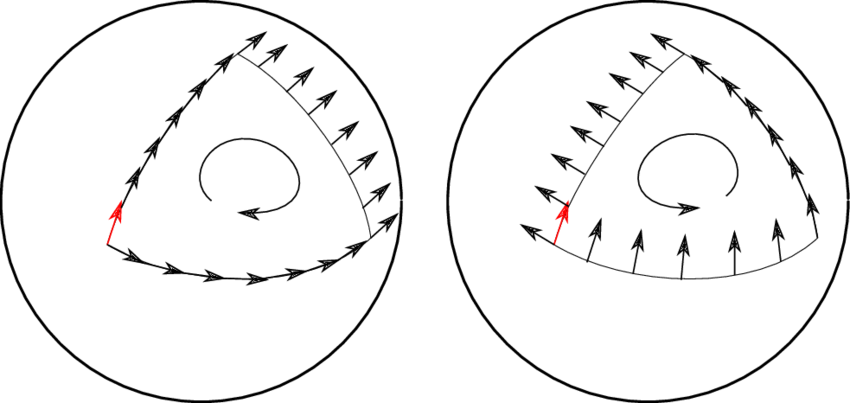
\includegraphics[width=0.60\textwidth]{parallel-transport.png}
	\caption{Parallel transport on a sphere.}
	\label{par-tr}
\end{figure}

\begin{proposition}
	La condizione di trasporto parallello di un campo vettoriale $ \ve{F}(\ve{x}) $ è che lungo la curva considerata si abbia $ \ve{e}^k \cdot d\ve{F} = 0 $.
\end{proposition}
Dato che $ d\ve{F} = \pa_l \ve{F} dx^l $, questa condizione è equivalente a richiedere che $ \nabla_l F^k = 0 $ lungo la curva.

\section{Derivata covariante}

Si introduce la seguente notazione per la derivata: $ f_{,i} = \frac{\pa f}{\pa x^i} $, indipendentemente dalla natura di $ f $.
Considerando un campo vettoriale $ \ve{F}(\ve{x}) $ su una varietà differenziabile $ \mathcal{M} $, quindi, si può riscrivere la derivata covariante come:
\begin{equation}
	\nabla_l F^k \equiv F^k_{;l} \defeq \ve{e}^k \cdot \ve{F}_{,l} = \ve{e}^k \cdot \left( F^i_{,l} \ve{e}_i + F^i \ve{e}_{i,l} \right) = F^k_{,l} + \Gamma^k_{li} F^i
	\label{eq:4.7}
\end{equation}

\begin{proposition}
	$ \ve{e}_k \cdot \ve{e}^i_{,l} = - \Gamma^i_{lk} $.
\end{proposition}
\begin{proof}
	$ 0 = \delta^i_{k,l} = \left( \ve{e}_k \cdot \ve{e}^i \right)_{,l} = \ve{e}_{k,l} \cdot \ve{e}^i + \ve{e}_k \cdot \ve{e}^i_{,l} = \Gamma^i_{lk} + \ve{e}_k \cdot \ve{e}^i_{,l} $.
\end{proof}
È dunque possibile esprimere la derivata covariante sia di un campo controvariante che di un campo covariante:
\begin{equation}
	V^k_{;l} \defeq \ve{e}^k \cdot \ve{V}_{,l} = \ve{e}^k \cdot \left( V^i_{,l} \ve{e}_i + V^i \ve{e}_{i,l} \right)
	\label{eq:4.8}
\end{equation}
\begin{equation}
	V_{k;l} \defeq \ve{e}_k \cdot \ve{V}_{,l} = \ve{e}_k \cdot \left( V_{i,l} \ve{e}^i + V_i \ve{e}^i_{,l} \right)
	\label{eq:4.9}
\end{equation}
Scrivendo in funzione delle connessioni affini:
\begin{equation}
	\nabla_l V^k = \frac{\pa V^k}{\pa x^l} + \Gamma^k_{li} V^i
	\label{eq:4.10}
\end{equation}
\begin{equation}
	\nabla_l V_k = \frac{\pa V_k}{\pa x^l} - \Gamma^i_{lk} V_i
	\label{eq:4.11}
\end{equation}
Sulle varietà torsion-free ($ T^a_{bc} \equiv 0 $) si può definire il rotore covariante come $ V_{l;i} - V_{i;l} = V_{l,i} - V_{i,l} $.

\begin{proposition}
	La derivata covariante trasforma come un tensore.
\end{proposition}
\begin{proof}
	Ricordando Eq. \ref{eq:4.6}:
	\begin{equation*}
		\begin{split}
			\tilde{\nabla}_l \tilde{V}^k
			&= \frac{\pa \tilde{V}^k}{\pa y^l} + \tilde{\Gamma}^k_{li}\tilde{V}^i = \frac{\pa x^m}{\pa y^l} \frac{\pa}{\pa x^m} \left( \frac{\pa y^k}{\pa x^p} V^p \right) + \tilde{\Gamma}^k_{lj} \tilde{V}^j\\
			&= \frac{\pa x^m}{\pa y^l} \frac{\pa y^k}{\pa x^p} \frac{\pa V^p}{\pa x^m} + \frac{\pa x^m}{\pa y^l} \frac{\pa^2 y^k}{\pa x^m \pa x^n} V^n + \frac{\pa y^k}{\pa x^p} \frac{\pa x^m}{\pa y^l} \underbrace{\frac{\pa x^n}{\pa y^j} \frac{\pa y^j}{\pa x_i}}_{\delta^n_i} \Gamma^p_{mn} V^i + \frac{\pa y^k}{\pa x^p} \frac{\pa^2 x^p}{\pa y^l \pa y^j} \frac{\pa y^j}{\pa x^n} V^n\\
			&= \frac{\pa x^m}{\pa y^l} \frac{\pa y^k}{\pa x^p} \left( \frac{\pa V^p}{\pa x^m} + \Gamma^p_{mn} V^n \right) + \left( \frac{\pa x^m}{\pa y^l} \frac{\pa^2 y^k}{\pa x^m \pa x^n} + \frac{\pa y^k}{\pa x^p} \frac{\pa^2 x^p}{\pa y^l \pa y^j} \frac{\pa y^j}{\pa x^n} \right) V^n
		\end{split}
	\end{equation*}
	Basta mostrare che il secondo termine è nullo:
	\begin{equation*}
		\begin{split}
			\frac{\pa}{\pa y^l} \frac{\pa y^k}{\pa x^n} + \frac{\pa y^k}{\pa x^p} \left[ \frac{\pa y^j}{\pa x^n} \frac{\pa}{\pa y^l} \frac{\pa x^p}{\pa y^j} \right]
			&= \frac{\pa}{\pa y^l} \frac{\pa y^k}{\pa x^n} + \frac{\pa y^k}{\pa x^p} \left[ \frac{\pa}{\pa y^l} \left( \frac{\pa y^j}{\pa x^n} \frac{\pa x^p}{\pa y^j} \right) - \frac{\pa x^p}{\pa y^j} \frac{\pa}{\pa y^l} \frac{\pa y^j}{\pa x^n} \right]\\
			&= \frac{\pa}{\pa y^l} \frac{\pa y^k}{\pa x^n} + \frac{\pa y^k}{\pa x^p} \left( \frac{\pa}{\pa y^l} \delta^p_n \right) - \delta^k_j \frac{\pa}{\pa y^l} \frac{\pa y^j}{\pa x^n} = \frac{\pa}{\pa y^l} \frac{\pa y^k}{\pa x^n} - \frac{\pa}{\pa y^l} \frac{\pa y^k}{\pa x^n} = 0
		\end{split}
	\end{equation*}
	Il caso della derivata covariante di un vettore covariante è analogo.
\end{proof}

\begin{proposition}\label{cov-2}
	La derivata covariante di un tensore di rango 2 è:
	\begin{equation}
		\nabla_k A_{ij} = \frac{\pa A_{ij}}{\pa x^k} - \Gamma^m_{ik} A_{mj} - \Gamma^m_{jk} A_{im}
		\label{eq:4.12}
	\end{equation}
	\begin{equation}
		\nabla_k A^{ij} = \frac{\pa A^{ij}}{\pa x^k} + \Gamma^i_{mk} A^{mj} + \Gamma^j_{mk} A^{im}
		\label{eq:4.13}
	\end{equation}
\end{proposition}
\begin{proof}
	$ \tens{A} = A_{ij} \ve{e}^i \otimes \ve{e}^j $, quindi:
	\begin{equation*}
		\begin{split}
			\frac{\pa \tens{A}}{\pa x^k}
			&= \frac{\pa A_{ij}}{\pa x^k} \ve{e}^i \otimes \ve{e}^j + A_{ij} \frac{\pa\ve{e}^i}{\pa x^k} \otimes \ve{e}^j + A_{ij} \ve{e}^i \otimes \frac{\pa\ve{e}^j}{\pa x^k}\\
			&= \frac{\pa A_{ij}}{\pa x^k} \ve{e}^i \otimes \ve{e}^j - A_{ij} \Gamma^i_{mk} \ve{e}^m \otimes \ve{e}^j - A_{ij} \Gamma^j_{mk} \ve{e}^i \otimes \ve{e}^m\\
			&= \frac{\pa A_{ij}}{\pa x^k} \ve{e}^i \otimes \ve{e}^j - A_{mj} \Gamma^m_{ik} \ve{e}^i \otimes \ve{e}^j - A_{im} \Gamma^m_{jk} \ve{e}^i \otimes \ve{e}^j\\
			&= \left( \frac{\pa A_{ij}}{\pa x^k} - \Gamma^m_{ik} A_{mj} - \Gamma^m_{jk} A_{im} \right) \ve{e}^i \otimes \ve{e}^j \eqdef \left( \nabla_k A_{ij} \right) \ve{e}^i \otimes \ve{e}^j
		\end{split}
	\end{equation*}
\end{proof}

\begin{proposition}
	Dato $ A_{ij} $ tensore di rango 2 antisimmetrico su una varietà torsion-free, si ha:
	\begin{equation}
		A_{ij;k} + A_{ki;j} + A_{jk;i} = A_{ij,k} + A_{ki,j} + A_{jk,i}
		\label{eq:4.14}
	\end{equation}
\end{proposition}
\begin{proof}
	Dalla Prop. \ref{cov-2}:
	\begin{equation*}
		\begin{split}
			A_{ij;k} + A_{ki;j} + A_{jk;i}
			&= A_{ij,k} - \Gamma^m_{ik} A_{mj} - \Gamma^m_{jk} A_{im} + A_{ki,j} - \Gamma^m_{kj} A_{mi} - \Gamma^m_{ij} A_{km} \\ &\qquad \qquad \qquad \qquad \qquad \qquad \qquad \qquad + A_{jk,i} - \Gamma^m_{ji} A_{mk} - \Gamma^m_{ki} A_{jm}
		\end{split}
	\end{equation*}
	Per simmetria di $ \Gamma^m_{ik} $ ed antisimmetria di $ A_{ij} $:
	\begin{equation*}
		\Gamma^m_{ik} A_{mj} = - \Gamma^m_{ki} A_{jk} \qquad \Gamma^m_{jk} A_{im} = - \Gamma^m_{kj} A_{mi} \qquad \Gamma^m_{ij} A_{km} = - \Gamma^m_{ji} A_{mk}
	\end{equation*}
	da cui segue la tesi.
\end{proof}

Ciò dimostra che l'identità di Bianchi è valida in qualsiasi sistema di riferimento su una varietà torsion-free.

\subsection{Varietà torsion-free}

\subsubsection{Connessioni affini}

\begin{definition}
	Si definisce \textit{simbolo di Christoffel del primo tipo} $ \Gamma_{ijk} \defeq g_{im} \Gamma^m_{jk} $.
\end{definition}

\begin{proposition}
	Su una varietà torsion-free $ \Gamma_{ijk} = \Gamma_{ikj} $.
\end{proposition}
\begin{proof}
	Banale ricordando che su una varietà torsion-free $ \Gamma^m_{jk} = \Gamma^m_{kj} $.
\end{proof}

\begin{proposition}\label{chri-1-2}
	$ \Gamma^m_{ij} = g^{km} \Gamma_{kij} $.
\end{proposition}
\begin{proof}
	$ g^{km} \Gamma_{kij} = g^{km} g_{kn} \Gamma^n_{ij} = \delta^m_n \Gamma^n_{ij} = \Gamma^m_{ij} $.
\end{proof}

È possibile esprimere le connessioni affini in funzione del tensore metrico.

\begin{proposition}\label{chri-1}
	$ \Gamma_{ijk} = \frac{1}{2} \left( g_{ij,k} + g_{ki,j} - g_{jk,i} \right) $.
\end{proposition}
\begin{proof}
	Si vede innanzitutto che $ \Gamma_{ijk} = g_{im} \Gamma^m_{jk} = g_{im} \ve{e}^m \cdot \ve{e}_{k,j} = \ve{e}_i \cdot \ve{e}_{k,j} $. Di conseguenza $ g_{ij,k} = \ve{e}_{i,k} \cdot \ve{e}_j + \ve{e}_i \cdot \ve{e}_{j,k} = \Gamma_{jki} + \Gamma_{ikj} $, ed analogamente $ g_{ki,j} = \Gamma_{ijk} + \Gamma_{kji} $ e $ g_{jk,i} = \Gamma_{kij} + \Gamma_{jik} $, dunque:
	\begin{equation*}
		\begin{split}
			g_{ij,k} + g_{ki,j} - g_{jk,i}
			&= \Gamma_{jki} + \Gamma_{ikj} + \Gamma_{ijk} + \Gamma_{kji} - \Gamma_{kij} - \Gamma_{jik}\\
			&= \Gamma_{jik} - \Gamma_{ijk} + \Gamma_{ijk} + \Gamma_{kij} - \Gamma_{kij} - \Gamma_{jik} = 2 \Gamma_{ijk}
		\end{split}
	\end{equation*}
\end{proof}

\begin{proposition}
	$ \Gamma^m_{ij} = \frac{1}{2} g^{km} \left( g_{ki,j} + g_{jk,i} - g_{ij,k} \right) $.
\end{proposition}
\begin{proof}
	Dalle Prop. \ref{chri-1-2} - \ref{chri-1}.
\end{proof}

\subsubsection{Derivata covariante del tensore metrico}

Dalla Prop. \ref{cov-2} si ha che:
\begin{equation}
	\nabla_k g_{ij} = \frac{\pa g_{ij}}{\pa x^k} - \Gamma^m_{ik} g_{mj} - \Gamma^m_{jk} g_{im}
	\label{eq:4.15}
\end{equation}
Dunque:
\begin{equation*}
	\begin{split}
		g_{ij;k}
		&= g_{ij,k} - \Gamma_{jik} - \Gamma_{ijk}\\
		&= g_{ij,k} - \frac{1}{2} \left( g_{ji,k} + g_{kj,i} - g_{ik,j} \right) - \frac{1}{2} \left( g_{ij,k} + g_{ki,j} - g_{jk,i} \right)\\
		&= g_{ij,k} - \frac{1}{2} g_{ijk,k} + \frac{1}{2} g_{jk,i} + \frac{1}{2} g_{ik,j} - \frac{1}{2} g_{ij,k} - \frac{1}{2} g_{ik,j} + \frac{1}{2} g_{jk,i} = 0
	\end{split}
\end{equation*}
Si vede quindi una delle proprietà fondamentali delle varietà torsion-free, ovvero la preservazione della metrica:
\begin{equation}
	\nabla_k g_{ij} = 0
	\label{eq:4.16}
\end{equation}

\section{Operatori differenziali su varietà curve}

Considerata una generica varietà differenziabile $ n $-dimensionale $ \mathcal{M} $, fissando un RF $ \{\ve{e}_i\}_{i = 1, \dots, n} $ ortogonale, è possibile definire su $ \mathcal{M} $ gli usuali operatori differenziali dello spazio euclideo.

\subsection{Gradiente}

\begin{definition}
	Dato  un campo scalare $ f : \mathcal{M} \rightarrow \R $, si definisce il suo differenziale come:
	\begin{equation}
		df(\ve{x}) = f(\ve{x} + d\ve{x}) - f(\ve{x}) = \frac{\pa f}{\pa x^i}dx^i \eqdef \nabla f(\ve{x}) \cdot d\ve{x}
		\label{eq:4.17}
	\end{equation}
\end{definition}

\begin{proposition}
	$ \nabla f = \displaystyle\sum_{i = 1}^{n} \frac{1}{h_i} \frac{\pa f}{\pa x^i} \hat{\ve{e}}_i $.
\end{proposition}
\begin{proof}
	Dato che $ \frac{\hat{\ve{e}}_i}{h_i} = \ve{e}^i $ (giustamente $ \frac{\pa f}{\pa x^i} $ è covariante):
	\begin{equation*}
		\nabla f \cdot d\ve{x} = \frac{\pa f}{\pa x^i} \ve{e}^i \cdot dx^j \ve{e}_j = \frac{\pa f}{\pa x^i} dx^j \delta^j_i = \frac{\pa f}{\pa x^i} dx^i = df
	\end{equation*}
\end{proof}

\subsection{Divergenza}

\begin{definition}
	Dato un campo vettoriale controvariante $ \ve{V} = V^i \ve{e}_i $, si definisce la sua divergenza come:
	\begin{equation}
		\nabla\cdot\ve{V} \defeq V^i_{;i} = V^i_{,i} + \Gamma^i_{ik} V^k
		\label{eq:4.18}
	\end{equation}
\end{definition}

La divergenza non è altro che una contrazione della derivata covariante.

\begin{proposition}\label{chri-contr}
	$ \Gamma^i_{ik} = \frac{1}{2} g^{im} g_{im,k} $.
\end{proposition}
\begin{proof}
	$ \Gamma^i_{ik} = \frac{1}{2} g^{im} \left( g_{im,k} + g_{ki,m} - g_{mk,i} \right) $, ma $ g^{im} g_{mk,i} = g^{mi} g_{ik,m} $ poichè $ m $, $ i $ indici muti, da cui la tesi.
\end{proof}

È possibile dare una formulazione alternativa. Si ricordi che, definendo $ c $ la matrice dei cofattori del tensore metrico $ g $ (visto come matrice):
\begin{equation}
	\det g = \sum_{i,j} g_{ij} c_{ij} \quad \Longrightarrow \quad c_{ij} = \frac{\pa\det g}{\pa g_{ij}}
	\label{eq:4.19}
\end{equation}
Ricordando poi che $ \left( g_{ij} \right)^{-1} = \left( \det g \right)^{-1} c_{ij} $:
\begin{equation}
	g^{ij} = \frac{1}{\det g} \frac{\pa\det g}{\pa g_{ij}}
	\label{eq:4.20}
\end{equation}

\begin{proposition}\label{chri-g}
	$ \Gamma^i_{ik} = \frac{\left( \sqg \right)_{,k}}{\sqg} $.
\end{proposition}
\begin{proof}
	Innanzitutto $ \left( \det g \right)_{,k} = g_{ij,k} \frac{\pa\det g}{\pa g_{ij}} = g_{ij,k} g^{ij} \det g $, quindi, dalla Prop. \ref{chri-contr}:
	\begin{equation*}
		\Gamma^i_{ik} = \frac{1}{2} g^{im} g_{im,k} = \frac{1}{2} \frac{1}{\det g} \left( \det g \right)_{,k} = \frac{1}{2\abs{\det g}} \abs{\det g}_{,k} \equiv \frac{\tens{g}_{,k}}{2\tens{g}} = \frac{\left( \sqg \right)_{,k}}{\sqg}
	\end{equation*}
\end{proof}

\begin{proposition}\label{dive-cov}
	Dato un campo vettoriale controvariante $ \ve{V} = V^i \ve{e}_i $, la sua divergenza è:
	\begin{equation}
		\nabla\cdot\ve{V} = \frac{\left( \sqg V^k \right)_{,k}}{\sqg}
		\label{eq:4.21}
	\end{equation}
\end{proposition}
\begin{proof}
	Dalle Prop. \ref{chri-g}:
	\begin{equation*}
		\nabla\cdot\ve{V} = V^i_{,i} + \Gamma^i_{ik} V^k = V^i_{,i} + \frac{\left( \sqg \right)_{,k}}{\sqg} V^k = \frac{\left( \sqg V^k \right)_{,k}}{\sqg}
	\end{equation*}
\end{proof}

\begin{definition}
	Si definisce la \textit{delta di Kronecker generalizzata} come:
	\begin{equation}
		\delta^{\mu_1 \dots \mu_k}_{\nu_1 \dots \nu_k} \defeq
		\begin{cases}
			+1 & (\nu_1,\dots,\nu_k) = \sigma_p (\mu_1,\dots,\mu_k) \text{ distinti} \\
			-1 & (\nu_1,\dots,\nu_k) = \sigma_d (\mu_1,\dots,\mu_k) \text{ distinti} \\
			0 & \text{altrimenti}
		\end{cases}
		\label{eq:4.22}
	\end{equation}
\end{definition}
\begin{lemma}
	Si ha:
	\begin{equation}
		\delta^{\mu_1 \dots \mu_k}_{\nu_1 \dots \nu_k} = \det
		\begin{bmatrix}
			\delta^{\mu_1}_{\nu_1} & \dots & \delta^{\mu_1}_{\nu_k}\\
			\vdots & \ddots & \vdots\\
			\delta^{\mu_k}_{\nu_1} & \dots & \delta^{\mu_k}_{\nu_k}
		\end{bmatrix}
		\label{eq:4.23}
	\end{equation}
\end{lemma}
\begin{lemma}\label{eps-gen}
	$ \epsilon_{i_1 \dots i_k i_{k+1} \dots i_n} \epsilon^{i_i \dots i_k j_{k+1} \dots j_n} = k! \delta^{j_{k+1} \dots j_n}_{i_{k+1} \dots i_n} $.
\end{lemma}

\begin{proposition}
	Dato un campo vettoriale $ \ve{V} = V^i \ve{e}_i $, detta $ V = V_i dx^i $ la forma differenziale ad esso associata, si ha:
	\begin{equation}
		\nabla\cdot\ve{V} = \sigma * d * V
		\label{eq:4.24}
	\end{equation}
\end{proposition}
\begin{proof}
	Per semplicità si considera il caso 4-dimensionale (si usa il Lemma \ref{eps-gen}):
	\begin{equation*}
		\begin{split}
			*d*V
			&= *d \left( V_i \frac{1}{3!} g^{ik} \varepsilon_{klmn} dx^l \wedge dx^m \wedge dx^n \right) = * \left[ \frac{1}{3!} \left( \sqg V^k \right)_{,p} \epsilon_{klmn} dx^p \wedge dx^l \wedge dx^m \wedge dx^n \right]\\
			&= \frac{1}{3!} \left( \sqg V^k \right)_{,p} \epsilon_{klmn} *\left( dx^p \wedge dx^l \wedge dx^m \wedge dx^n \right) = \frac{1}{3!} \left( \sqg V^k \right)_{,p} \epsilon_{klmn} g^{p \alpha} g^{l \beta} g^{m \gamma} g^{n \delta} \sqg \epsilon_{\alpha \beta \gamma \delta}\\
			&= \frac{1}{3!} \left( \sqg V^k \right)_{,p} \sqg \epsilon_{klmn} \left( \det g \right)^{-1} \epsilon^{plmn} = \frac{1}{3!} \frac{\sigma}{\sqg} \left( \sqg V^k \right)_{,p} \left( 3! \delta^p_k \right) = \frac{\sigma}{\sqg} \left( \sqg V^k \right)_{,k}
		\end{split}
	\end{equation*}
\end{proof}

\begin{example}
	In uno spazio piatto $ n $-dimensionale con $ g_{ij} = h_i^2 \delta_{ij} $ si ha $ \bar{V}_i \equiv h_i^{-1} V_i = h_i V^i $, quindi:
	\begin{equation*}
		\nabla\cdot\ve{V} = \frac{1}{\sqrt{h_1^2 \dots h_n^2}} \sum_{k = 1}^{n} \left( \sqrt{h_1^2 \dots h_n^2} \bar{V}_k \right)_{,k} = \frac{1}{h_1 \dots h_n} \sum_{k = 1}^{n} \frac{\pa}{\pa x^k} \left( \frac{h_1 \dots h_n}{h_k} V_k \right)
	\end{equation*}
\end{example}

\subsection{Laplaciano}

\begin{definition}
	Dato un campo scalare $ f : \mathcal{M} \rightarrow \R $, si definisce il suo laplaciano come:
	\begin{equation}
		\Box f \defeq \nabla\cdot\nabla f = \left( g^{ik} f_{,k} \right)_{;i}
		\label{eq:4.25}
	\end{equation}
\end{definition}

% Nella letteratura russa è indicato anche con $ \Delta $, mentre in uno spazio piatto con $ \nabla^2 $.

\begin{proposition}
	Si ha:
	\begin{equation}
		\Box f = \frac{\left( \sqg f^{,k} \right)_{,k}}{\sqg}
		\label{eq:4.26}
	\end{equation}
\end{proposition}
\begin{proof}
	Banale dalla Prop. \ref{dive-cov}, usando $ g^{ik} f_{,k} = f^{,i} $.
\end{proof}

\begin{proposition}
	Dato un campo scalare $ f : \mathcal{M} \rightarrow \R $, si ha:
	\begin{equation}
		\Box f = \sigma * d * df
		\label{eq:4.27}
	\end{equation}
\end{proposition}
\begin{proof}
	\begin{equation*}
		\begin{split}
			*d*df
			&= *d \left( f_{,i} *dx^i \right) = *d \left( \frac{1}{3!} \sqg f_{,i} g^{ik} \epsilon_{klmn} dx^l \wedge dx^m \wedge dx^n \right)\\
			&= * \left( \frac{1}{3!} \left( \sqg f^{,k} \right)_{,p} \epsilon_{klmn} dx^p \wedge dx^l \wedge dx^m \wedge dx^n \right)\\
			&= \frac{1}{3!} \left( \sqg f^{,k} \right)_{,p} \epsilon_{klmn} g^{p \alpha} g^{l \beta} g^{m \gamma} g^{n \delta} \sqg \epsilon_{\alpha \beta \gamma \delta}\\
			&= \frac{1}{3!} \left( \sqg f^{,k} \right)_{,p} \epsilon_{klmn} \sqg \left( \det g \right)^{-1} \epsilon^{plmn} = \frac{1}{3!} \frac{\sigma}{\sqg} \left( \sqg f^{,k} \right)_{,p} 3! \delta^p_k = \frac{\sigma}{\sqg} \left( \sqg f^{,k} \right)_{,k}
		\end{split}
	\end{equation*}
\end{proof}

\begin{example}
	In uno spazio piatto $ n $-dimensionale con $ g_{ij} = h_i^2 \delta_{ij} $ si ha $ f^{,k} = g^{ik} f_{,i} = h_k^{-2} f_{,k} $, quindi:
	\begin{equation*}
		\nabla^2 f = \frac{1}{\sqrt{h_1^2 \dots h_n^2}} \sum_{k = 1}^{n} \left( \sqrt{h_1^2 \dots h_n^2} h_k^{-2} f_{,k} \right)_{,k} = \frac{1}{h_1 \dots h_n} \sum_{k = 1}^{n} \frac{\pa}{\pa x^k} \left( \frac{h_1 \dots h_n}{h_k^2} \frac{\pa f}{\pa x^k} \right)
	\end{equation*}
\end{example}

\section{Elettrodinamica covariante}

Riprendendo il potenziale \ref{eq:2.21}, è possibile definire la 1-form $ A = A_i dx^i $:

\begin{equation}
	dA = \pa_i A_j dx^i \wedge dx^j = \frac{1}{2} F_{ij} dx^i \wedge dx^j \equiv F
	\label{eq:3.13}
\end{equation}

dove è stata definita la 2-form determinata dal tensore di Faraday \ref{eq:2.23}. L'Eq. \ref{eq:2.25} diventa, grazie all'identità di Bianchi:

\begin{equation}
	dF = 0
	\label{eq:3.14}
\end{equation}

Nel caso elettrostatico $ \dot{\ve{B}} = 0 $, quindi $ \nabla\times\ve{E} = 0 $, ovvero $ dE = 0 $: il campo elettrostatico è chiuso e, per il teorema di Stokes, localmente esatto.\\
È anche possibile calcolare il duale di Hodge di $ F $:
\begin{equation}
	*F = \frac{1}{2}F_{ij} * \left( dx^i \wedge dx^j \right) = \frac{1}{4} F_{ij} g^{ik} g^{il} \varepsilon_{klmn} dx^m \wedge dx^n = \frac{1}{4} F^{kl} \varepsilon_{klmn} dx^m \wedge dx^n
	\label{eq:3.22}
\end{equation}
Applicando il duale della derivata esteriore:
\begin{equation}
	\begin{split}
		*d*F &= \frac{1}{4} \pa_p \left( F^{kl} \varepsilon_{klmn} \right) * \left( dx^p \wedge dx^m \wedge dx^n \right) = \frac{1}{4} \pa_p \left( \sqg F^{kl} \right) \epsilon_{klmn} g^{p\alpha} g^{m\beta} g^{n\gamma} \varepsilon_{\alpha\beta\gamma\delta} dx^{\delta}\\
		     &= \frac{1}{4} \pa_p \left( \sqg F^{kl} \right) \sqg \, \epsilon_{klmn} g^{\alpha p} g^{\beta m} g^{\gamma n} g^{\delta w} \epsilon_{\alpha\beta\gamma\delta} dx_w = \frac{1}{4} \pa_p \left( \sqg F^{kl} \right) \sqg\, \epsilon_{klmn} \frac{\sigma}{\tens{g}} \epsilon^{pmnw} dx_w\\
		     &= \frac{1}{4} \pa_p \left( \sqg F^{kl} \right) \frac{\sigma}{\sqg} 2 \left( \delta^p_k \delta^w_l - \delta^w_k \delta^p_l \right) dx_w = \frac{\sigma}{2\sqg} \left[ \pa_p \left( \sqg F^{pw} \right) dx_w - \pa \left( \sqg F^{wp} \right) dx_w \right]\\
		     &= - \frac{\sigma}{\sqg} \pa_p \left( \sqg F^{kp} \right) dx_k
	\end{split}
	\label{eq:3.23}
\end{equation}
Nello spaziotempo di Minkowski $ g_{ij} = \diag(-1,1,1,1) $, dunque l'Eq. \ref{eq:3.23} si riduce a $ *d*F = \pa_p (F^{kp}) dx_k $: ricordando dall'Eq. \ref{eq:2.27} che $ \pa_p (F^{kp}) = \mu_0 j^k $, definendo la 1-form della corrente $ j \defeq j^k dx_k $ si trova la generalizzazione su varietà curva della seconda equazione di Maxwell covariante:
\begin{equation}
	*d*F = \mu_0 j
	\label{eq:3.24}
\end{equation}
Questa, unità all'identità di Bianchi Eq. \ref{eq:3.14}, rappresenta tutti i fenomeni dell'elettrodinamica classica.












\chapter{Principio d'Equivalenza}
\selectlanguage{italian}

\section{Principio d'azione stazionaria}

\subsection{Caso classico}

\begin{definition}
	Dato un sistema descritto da una lagrangiana $ L $, si definisce l'azione come:
	\begin{equation}
		S[\ve{x}(t)] \defeq \int_{t_1}^{t_2} L(\ve{x}, \dot{\ve{x}}) dt
		\label{eq:5.1}
	\end{equation}
\end{definition}

Il principio di minima azione afferma che la traiettoria percorsa dal sistema è un estremante dell'azione, ovvero, considerata una variazione della traiettoria $ \delta\ve{x} : \delta\ve{x}(t_1) = \delta\ve{x}(t_2) = \ve{0} $:
\begin{equation}
	\delta S = 0
	\label{eq:5.2}
\end{equation}

\paragraph{Particella libera}

Classicamente, una particella libera è descritta da $ L = \frac{1}{2} m \dot{\ve{x}}^2 $, dunque:
\begin{equation*}
	\begin{split}
		0
		&= \delta S = \int_{t_1}^{t_2} \delta L \,dt = \int_{t_1}^{t_2} m \dot{\ve{x}} \cdot \delta\dot{\ve{x}} \,dt = \int_{t_1}^{t_2} \left[ m \frac{d}{dt} \left( \dot{\ve{x}} \cdot \delta\ve{x} \right) - m \ddot{\ve{x}} \cdot \delta\ve{x} \right] dt\\
		&= m \left[ \ddot{\ve{x}} \cdot \delta\ve{x} \right]_{t_1}^{t_2} - m \int_{t_1}^{t_2} \ddot{\ve{x}} \cdot \delta\ve{x} \,dt = -m \int_{t_1}^{t_2} \ddot{\ve{x}} \cdot \delta\ve{x} \,dt
	\end{split}
\end{equation*}
Dunque, data l'arbitrarietà di $ \delta\ve{x} $, si ha l'equazione del moto della particella libera classica:
\begin{equation}
	\ddot{\ve{x}} = \ve{0}
	\label{eq:5.3}
\end{equation}

\paragraph{Moto in un potenziale}

In presenza di un potenziale, la lagrangiana diventa $ L = \frac{1}{2} m \dot{\ve{x}}^2 - V(\ve{x}) $, quindi, dato che $ \delta V(\ve{x}) = \nabla V(\ve{x}) \cdot \delta\ve{x} $, si ha l'equazione del moto:
\begin{equation}
	0 = \delta S = \int_{t_1}^{t_2} \left( - m\ddot{\ve{x}} - \nabla V(\ve{x}) \right) \cdot \delta\ve{x} \,dt \quad\Longrightarrow\quad m\ddot{\ve{x}} = - \nabla V(\ve{x})
	\label{eq:5.4}
\end{equation}

\subsection{Caso relativistico}

\begin{proposition}
	Una particella libera relativistica è descritta da $ L = - \frac{m c^2}{\gamma} $.
\end{proposition}
\begin{proof}
	$ p_i = \frac{\pa L}{\pa v_i} = - mc^2 \frac{\pa}{\pa v_i} \sqrt{1 - \frac{\ve{v}^2}{c^2}} = -mc^2 \left( -  \gamma \frac{v_i}{c} \right) = \gamma m v_i $, ovvero $ \ve{p} = \gamma m \ve{v} $.
\end{proof}

\paragraph{Particella libera}

L'azione che descrive una particella libera relativistica è:
\begin{equation}
	S = - mc^2 \int_{t_1}^{t_2} \frac{dt}{\gamma} = -mc \int_{\tau_1}^{\tau_2} d\tau
	\label{eq:5.5}
\end{equation}
Ponendo $ c = 1 $, è possibile calcolare le equazioni del moto:
\begin{equation*}
	\begin{split}
		0
		&= \delta S = - \delta \int_{t_1}^{t_2} m \sqrt{1 - \dot{\ve{x}}^2} \,dt = m \int_{t_1}^{t_2} \frac{\dot{\ve{x}} \cdot \delta\dot{\ve{x}}}{\sqrt{1 - \dot{\ve{x}}^2}} dt = m \int_{t_1}^{t_2} \frac{d\ve{x}}{dt} \cdot \frac{d \delta\ve{x}}{dt} \frac{dt}{d\tau} \,dt\\
		&= m \int_{\tau_1}^{\tau_2} \frac{d\ve{x}}{dt} \cdot \frac{d \delta\ve{x}}{dt} \frac{dt}{d\tau} \frac{dt}{d\tau} \,d\tau = m \int_{\tau_1}^{\tau_2} \frac{d\ve{x}}{d\tau} \cdot \frac{d\delta\ve{x}}{d\tau} \,d\tau\\
		&= m \int_{\tau_1}^{\tau_2} \left[ \frac{d}{d\tau} \left( \dot{\ve{x}} \cdot \delta\ve{x} \right) - \frac{d^2\ve{x}}{d\tau^2} \cdot \delta\ve{x} \right] d\tau = - m \int_{\tau_1}^{\tau_2} \frac{d^2 \ve{x}}{d\tau^2} \cdot \delta\ve{x} \,d\tau
	\end{split}
\end{equation*}
Dall'arbitrarietà di $ \delta\ve{x} $ si ottiene l'equazione del moto:
\begin{equation}
	\frac{d^2 \ve{x}}{d\tau^2} = \ve{0}
	\label{eq:5.6}
\end{equation}

\paragraph{Campo elettromagnetico}

Per descrivere il moto di una particella in un campo elettromagnetico, è necessario aggiungere un termine d'interazione alla lagrangiana:
\begin{equation}
	S = -m \int_{\tau_1}^{\tau_2} d\tau + q \int_{\ve{x}_1}^{\ve{x}_2} A_i(\ve{x}) dx^i = \int_{\tau_1}^{\tau_2} \left( -m + q A_i (\ve{x}) \frac{dx^i}{d\tau} \right) d\tau
	\label{eq:5.7}
\end{equation}
Per ottenere le equazioni del moto, dunque:
\begin{equation*}
	\begin{split}
		0
		&= \delta S = -m \int_{\tau_1}^{\tau_2} \delta\sqrt{-\eta_{ij} dx^i dx^j} + q \int_{\ve{x}_1}^{\ve{x}_2} \delta \left( A_i dx^i \right)\\
		&= -m \int_{\tau_1}^{\tau_2} \frac{1}{2} \frac{\delta \left( - \eta_{ij} dx^i dx^j \right)}{\sqrt{- \eta_{ij} dx^i dx^j}} + q \int_{\ve{x}_1}^{\ve{x}_2} \left( \delta A_i dx^i + A_i \delta dx^i \right)\\
		&= m \int_{\tau_1}^{\tau_2} \frac{1}{2} \frac{\eta_{ij} \left( \delta dx^i dx^j + dx^i \delta dx^j \right)}{\sqrt{- \eta_{ij} dx^i dx^j}} + q \int_{\tau_1}^{\tau_2} \left( \delta A_i \frac{dx^i}{d\tau} + A_i \frac{d\delta x^i}{d\tau} \right) d\tau\\
		&= \int_{\tau_1}^{\tau_2} \left( m \frac{\eta_{ij} dx^i}{\sqrt{- \eta_{ij} dx^i dx^j}} \frac{d\delta x^j}{d\tau} + q \frac{\pa A_i}{\pa x^k} \delta x^k \frac{dx^i}{d\tau} + q A_i \frac{d\delta x^i}{d\tau} \right) d\tau\\
		&= \int_{\tau_1}^{\tau_2} \left( m \eta_{ij} \frac{dx^i}{d\tau} \frac{d\delta x^j}{d\tau} + q A_{i,k} \delta x^k \frac{dx^i}{d\tau} + q A_i \frac{d\delta x^i}{d\tau} \right) d\tau\\
		&= \int_{\tau_1}^{\tau_2} \left( - m \frac{du_k}{d\tau} \delta x^k + q A_{i,k} u^i \delta x^k - q \frac{dA_k}{d\tau} \delta x^k \right) d\tau\\
		&= \int_{\tau_1}^{\tau_2} \left( -m \frac{du_k}{d\tau} + q \left( A_{i,k} - A_{k,i} \right) u^i \right) \delta x^k d\tau
	\end{split}
\end{equation*}
dove si è usata la quadrivelocità $ u_k $. Ricordando la definizione del tensore di Faraday $ F_{ij} \defeq A_{j,i} - A_{i,j} $, si trova l'espressione covariante della forza di Lorentz:
\begin{equation}
	\frac{dp_k}{d\tau} = q F_{ki} u^i
	\label{eq:5.8}
\end{equation}
Ciò conferma la scelta della lagrangiana.

\paragraph{Campo gravitazionale}

Si consideri ora una particella su una varietà curva:
\begin{equation*}
	\begin{split}
		0
		&= \delta S = -m \int_{\tau_1}^{\tau_2} \delta d\tau = -m \int_{\tau_1}^{\tau_2} \delta \sqrt{- g_{ij} dx^i dx^j} = m \int_{\tau_1}^{\tau_2} \frac{1}{2} \frac{\delta g_{ij} dx^i dx^j + 2g_{ij} dx^i \delta dx^j}{\sqrt{- g_{ij} dx^i dx^j}}\\
		&= m \int_{\tau_1}^{\tau_2} \left( \frac{1}{2} g_{ij,k} u^i u^j \delta x^k d\tau + g_{ij} u^i \delta dx^j \right) = m \int_{\tau_1}^{\tau_2} \left( \frac{1}{2} g_{ij,k} u^i u^j \delta x^k + g_{ij} u^i \frac{d\delta x^j}{d\tau} \right) d\tau\\
		&= m \int_{\tau_1}^{\tau_2} \left( \frac{1}{2} g_{ij,k} u^i u^j \delta x^k - \frac{d}{d\tau} \left( g_{ij} u^i \right) \delta x^j \right) d\tau = m \int_{\tau_1}^{\tau_2} \left( \frac{1}{2} g_{ij,k} u^i u^j - \frac{d}{d\tau} \left( g_{ik} u^i \right) \right) \delta x^k d\tau
	\end{split}
\end{equation*}
Essendo $ \delta x^k $ arbitrario si ottiene:
\begin{equation}
	\frac{1}{2} g_{ij,k} u^i u^j - g_{ik,j} u^i u^j - g_{ik} \frac{du^i}{d\tau} = 0
	\label{eq:5.9}
\end{equation}
Moltiplicando per $ g^{rk} $:
\begin{equation}
	\frac{du^r}{d\tau} + g^{rk} \left( g_{ik,j} - \frac{1}{2} g_{ij,k} \right) u^i u^j = 0
	\label{eq:5.10}
\end{equation}
Dato che sopravvive solo la parte simmetrica rispetto a $ i,j $ del tensore moltiplicato per $ u^i u^j $:
\begin{equation}
	\frac{du^r}{d\tau} + \frac{1}{2} g^{rk} \left( g_{ik,j} + g_{jk,i} - g_{ij,k} \right) u^i u^j = 0
	\label{eq:5.11}
\end{equation}
Si vede la definizione di connessione di Levi-Civita (Eq. \ref{levi-civita}):
\begin{equation}
	\frac{d^2 x^r}{d\tau^2} + \Gamma^r_{ij} \frac{dx^i}{d\tau} \frac{dx^j}{d\tau} = 0
	\label{eq:5.12}
\end{equation}
Questa è nota come \textit{equazione geodetica} e descrive il moto di una particella libera su una varietà curva: si vede che, oltre al termine inerziale, è presente un termine di forza dovuto alla geometria stessa dello spazio; inoltre, si può osservare come la traiettoria sia indipendente dalla massa del corpo.
Sebbene la connessione di Levi-Civita non sia un tensore, si dimostra che il termine di forza annulla i termini non-omogenei, rendendo l'equazione geodesica un'equazione tensoriale.

\paragraph{Campo elettromagnetico e gravitazionale}

Nel caso di una particella soggetta ad un campo elettromagnetico su una varietà curva:
\begin{equation}
	S = -m \int_{\tau_1}^{\tau_2} \sqrt{- g_{ij} dx^i dx^j} + q \int_{\tau_1}^{\tau_2} A_i \frac{dx^i}{d\tau} d\tau
	\label{eq:5.13}
\end{equation}
Svolgendo i calcoli, si trova l'equazione del moto:
\begin{equation}
	\frac{d^2 x^r}{d\tau^2} + \Gamma^r_{ij} \frac{dx^i}{d\tau} \frac{dx^j}{d\tau} - \frac{q}{m} F^r_{\,\,\,i} \frac{dx^i}{d\tau} = 0
	\label{eq:5.14}
\end{equation}
che conferma l'identificazione del termine geometrico con la forza di gravità.












\end{document}
